\documentclass[oneside]{book}

\usepackage[english,spanish]{babel}
\usepackage[utf8]{inputenc}
\usepackage{amsthm}
\usepackage{amsmath}
\usepackage[pdftex]{graphicx}
\usepackage{epstopdf}
\usepackage{enumerate}
\usepackage[lite]{mtpro2}
\usepackage[absolute]{textpos}
\usepackage{tabularx}
\usepackage{setspace}
\usepackage{float}
\usepackage[fixlanguage]{babelbib}
\usepackage{bibentry}
\usepackage{fancyvrb}

\title{Programación de sistemas multi-agente utilizando argumentacion} % do change
\author{Leonardo Molas}

\setlength{\parskip}{0.5\baselineskip}

\renewcommand{\topfraction}{0.85}
\renewcommand{\textfraction}{0.1}

\renewcommand{\floatpagefraction}{0.75}

\setbtxfallbacklanguage{english}
\selectbiblanguage{spanish}

% package float: bordes
\floatstyle{ruled} 
\restylefloat{figure}

\theoremstyle{definition}
\newtheorem{definicion}{Definición}[section]

\newcommand{\ie}{i.\,e.}
\newcommand{\etal}{\mbox{{\em et al.}}}
\newcommand{\eg}{e.\,g.}
\newcommand{\raya}{\rule{\textwidth}{.05mm}}
\newcommand{\eoe}{\begin{flushright}$\Box$\end{flushright}}
\newcommand{\marginnote}[1]{\marginpar{\frame{#1}}}
\newcommand{\new}{\marginpar{\frame{\sc new}}}


\newcommand{\DLP}{\mbox{\textit{DeLP}}}
\newcommand{\DLPa}{\mbox{DeLP}}
\newcommand{\DLPas}{\mbox{DeLP(a)-strict}}
\newcommand{\DLPans}{\mbox{DeLP(a)-non-strict}}
\newcommand{\dlp}{\mbox{\it de.l.p.}}

\newcommand{\cree}{B}

\newcommand{\no}{\mbox{$\sim$}}
\newcommand{\negda}[1]{\mbox{\textsf{not}$#1$}}
\newcommand{\naf}{\p{$\backslash$+}}
\newcommand{\notj}{{not}}
%\newcommand{\comp}[1]{\mbox{$\overline{#1}$}}
\newcommand{\simbcomp}{ $\stackrel{\comp{\ \ }}{\vrule width 0pt height.8ex}$ }

\newcommand{\p}[1]{{\small \tt #1}}

% DLP programs 
% strict rule
\newcommand{\srule}[2]{\mbox{$ #1\;\leftarrow\;#2$}}
%\newcommand{\fact}[1]{\mbox{$ #1$}}  % some cls files have \fact defined for other things 
\newcommand{\facto}[1]{\mbox{$ #1$}} % for compatibility when the reason above holds
% literal
\newcommand{\lit}[1]{\mbox{$ #1$}}
% defesible rule
\newcommand{\drule}[2]{\mbox{$ #1\; \defleftarrow \; #2$}}
\newcommand{\defleftarrow}{{\raise1.5pt\hbox{\tiny\defleft}}}
\newcommand{\defleft}{\mbox{---\hspace{-1.5pt}\raise.05pt\hbox{$<$}}}
% presumption
%\newcommand{\presum}[1]{\drule{#1}{true}}
\newcommand{\presum}[1]{\drule{#1}{}}
% inverted rules
\newcommand{\invleftarrow}{ $\hookleftarrow $ }
\newcommand{\irule}[2]{\mbox{$#1$ \invleftarrow $#2$}}
\newcommand{\dquery}[1]{\drule{}{#1}}

% Donald Nute rules
\newcommand{\rr}[2]{\mbox{$ #1 \Rightarrow #2 $}} % defeasible
\newcommand{\re}[2]{\mbox{$#1 \rightarrow #2 $}} % strict
\newcommand{\de}[2]{\mbox{$ #1 \leadsto #2$}} %defeater

% Programci�n en Logica Extendida
\newcommand{\ple}{\mbox{\sc PLE}}
\newcommand{\extclause}[2]{\mbox{ #1 $\leftarrow$ #2}}
\newcommand{\true}{$true$}

% flecha rebatible para la derecha
\newcommand{\defrightarrow}{\mbox{$\succ\!$---}}
\newcommand{\defarrow}{{\raise1.5pt\hbox{\tiny\defrightarrow}}}


% Argumentos
\newcommand{\ArgA}{\mbox{${\mathcal A}$}}
\newcommand{\Ap}{\mbox{\ArgA$'$}}
\newcommand{\ArgAo}{\mbox{${\mathcal A_0}$}}
\newcommand{\ArgAa}{\mbox{${\mathcal A_1}$}}
\newcommand{\ArgAb}{\mbox{${\mathcal A_2}$}}
\newcommand{\ArgAn}{\mbox{${\mathcal A_n}$}}
\newcommand{\ArgAi}{\mbox{${\mathcal A_i}$}}
\newcommand{\ArgAim}{\mbox{${\mathcal A_{i-1}}$}}
\newcommand{\ArgB}{\mbox{${\mathcal B}$}}
\newcommand{\ArgBo}{\mbox{${\mathcal B_0}$}}
\newcommand{\ArgBa}{\mbox{${\mathcal B_1}$}}
\newcommand{\ArgBb}{\mbox{${\mathcal B_2}$}}
\newcommand{\ArgBk}{\mbox{${\mathcal B_k}$}}
\newcommand{\ArgQ}{\mbox{${\mathcal Q}$}}
\newcommand{\ArgQo}{\mbox{${\mathcal Q_0}$}}
\newcommand{\ArgQa}{\mbox{${\mathcal Q_1}$}}
\newcommand{\ArgQb}{\mbox{${\mathcal Q_2}$}}
\newcommand{\ArgQk}{\mbox{${\mathcal Q_k}$}}
\newcommand{\ArgQn}{\mbox{${\mathcal Q_n}$}}
\newcommand{\ArgQi}{\mbox{${\mathcal Q_i}$}}
\newcommand{\ArgQim}{\mbox{${\mathcal Q_{i-1}}$}}
\newcommand{\AQ}{\mbox{$\langle \ArgA,\ArgQ \rangle $}}
\newcommand{\AoQo}{\mbox{$\langle \ArgAo,\ArgQo \rangle $}}
\newcommand{\AaQa}{\mbox{$\langle \ArgAa,\ArgQa \rangle $}}
\newcommand{\AbQb}{\mbox{$\langle \ArgAb,\ArgQb \rangle $}}
\newcommand{\AnQn}{\mbox{$\langle \ArgAn,\ArgQn \rangle $}}
\newcommand{\AiQi}{\mbox{$\langle \ArgAi,\ArgQi \rangle $}}
\newcommand{\AimQim}{\mbox{$\langle \ArgAim,\ArgQim \rangle $}}
\newcommand{\BaQa}{\mbox{$\langle \ArgBa,\ArgQa \rangle $}}
\newcommand{\BkQk}{\mbox{$\langle \ArgBk,\ArgQk \rangle $}}

\newcommand{\Argum}[2]{\mbox{$\langle #1, #2 \rangle $}}
\newcommand{\AS}[2]{$\langle \{#1\}, #2 \rangle $}
\newcommand{\bigAS}[2]{$\bigl\langle \{#1\}, #2 \bigr\rangle $}

\newcommand{\nlA}[1]{$$\mbox{#1}$$}

% Sets of rules
\newcommand{\Facts}{\mbox{$\Theta$}}       % Facts
\newcommand{\SRules}{\mbox{$\Omega$}}       % Stricts rules
\newcommand{\SSet}{\mbox{$\Pi$}}       % Stricts rules & facts
\newcommand{\SSg}{\mbox{${\SSet}_G$}}  % Stricts rules without facts 
\newcommand{\SSp}{\mbox{${\SSet}_P$}}  % set of facts
\newcommand{\DD}{\mbox{$\Delta$}}      % Defeasible rules
\newcommand{\SD}{\mbox{$(\SSet,\DD)$}} % sets of rules of a program 
\newcommand{\FSD}{\mbox{$(\Facts,\SRules,\DD)$}} % sets of rules of a program 
\newcommand{\Presumptions}{\mbox{$\Phi$}}   % 
\newcommand{\DDp}{\mbox{$\Delta^{+}$}}  % Defeasible rules and presumptions
\newcommand{\SDp}{\mbox{$(\SSet,\DDp)$}} % sets of rules of a program 
\newcommand{\FSDP}{\mbox{$(\Facts,\SRules,\DD,\Presumptions)$}} % sets of rules of a program 

\newcommand{\FySyD}{\mbox{\Facts\ $\cup$ \SSet\ $\cup$ \DD}}   
\newcommand{\SyD}{\mbox{\SSet\ $\cup$ \DD}}   
\newcommand{\SyA}{\mbox{\SSet\ $\cup$ \ArgA}}
\newcommand{\SyAp}{\mbox{\SSet\ $\cup$ \Ap}}
\newcommand{\SyArga}{\mbox{\SSet\ $\cup$ \Arga}}
\newcommand{\RR}{\mbox{$\mathcal R$}}
\newcommand{\PP}{\mbox{${\mathcal P}$}}
\newcommand{\PPa}{\mbox{${\mathcal P}_1$}}
\newcommand{\PPb}{\mbox{${\mathcal P}_2$}}
\newcommand{\PPc}{\mbox{${\mathcal P}_3$}}
\newcommand{\PPd}{\mbox{${\mathcal P}_4$}}
\newcommand{\FFi}{\mbox{${\mathcal F}_i$}}
\newcommand{\FF}{\mbox{${\mathcal F}$}}

% nuevos comanditos
\newcommand{\SyQaQ}{\mbox{$\SSet \cup \{\ArgQa\\,\ArgQ\}$}}

\newcommand{\SDC}{\mbox{$(\SSet,\DD,\preceq)$}} 
\newcommand{\cquery}[2]{\mbox{$[#1,#2]$}}
\newcommand{\addset}{\mbox{$\Phi^+$}}
\newcommand{\remset}{\mbox{$\Theta^-$}}
\newcommand{\BB}{\mathcal{PB}}
\newcommand{\SB}{\SSet^B}
\newcommand{\DB}{\DD^B}
\newcommand{\CCB}{\CC^B}


\newcommand{\GB}{\mathcal{PG}}
\newcommand{\SG}{\SSet^G}
\newcommand{\DG}{\DD^G}
\newcommand{\CCG}{\CC^G}
\newcommand{\EG}{E_G}
\newcommand{\CG}{\CC_G}


\newcommand{\hugo}[1]{\mbox{$#1$}\xspace}
\newcommand{\K}{\mathcal{K}}
\newcommand{\DeLPK}{\DLP\ Knowledge Base}
\newcommand{\External}{External Knowledge Base}
\newcommand{\eLit}[2]{#1_#2}
\newcommand{\co}[1]{Co(#1)}

\newcommand{\CC}{\hugo{\prec}}
\newcommand{\CCe}{\hugo{\CC_{GE}}}

\begin{document}

% \maketitle

% parte robada de los chicos

\thispagestyle{empty}

\begin{textblock*}{10cm} (6cm,8cm) % {ancho} {X, Y}
\begin{center}
\begin{tabular}{c}
{\LARGE Programación de sistemas multi-agente utilizando argumentacion	} \\
\\
Leonardo Molas (LU: 82498)\\
Juan Manuel Torres (LU: 83410)\\
\\
Director: \emph{Dr. Diego Martínez}\\
\\
%\date
\end{tabular}
\end{center}
\end{textblock*}
\null
\vfill
\pagebreak
\thispagestyle{empty}

\setcounter{page}{1}
%fin


\tableofcontents

\chapter*{Introducción}

\addcontentsline{toc}{chapter}{Introducción}

El grupo de investigación del Laboratorio de Investigación y Desarrollo en 
Inteligencia Artificial (LIDIA) fue creado en 1992 en la Universidad Nacional 
del Sur. En el año 2011, un conjunto de sus integrantes decidió conformar un 
equipo de desarrollo \cite{Garay12} con el objetivo de participar en el concurso de programación 
Multi-Agent Programming Contest 2011 (MAPC). El equipo que diseñó el sistema 
\texttt{d3lp0r}\ estuvo compuesto
por los profesores Guillermo Simari, Diego Martínez y Alejandro García, el Doctor
Sebastián Gottifredi, y los estudiantes de grado Leonardo Molas, 
Juan Manuel Torres, Diego Marcovecchio, Iñaki Garay, Fernando Sisul y Emiliano Montenegro.
Estos últimos fueron los encargados del desarrollo del sistema, mientras que tanto
los profesores como el Dr. Gottifredi fueron fuente de consulta y orientación
para los desarrolladores.
	
La motivación principal del equipo consistió en aplicar argumentación \cite{Prakken:1997} 
\cite{Rahwan:2009} \cite{Bench-Capon:2007}\ mediante programación lógica rebatible (\DLP
\cite{Garcia:2004a}) en un agente basado en la arquitectura \textit{BDI} \cite{Amgoud:2008}. Esto
fue aplicado en el contexto de un sistema multi-agente que opera en un ambiente dinámico
y competitivo como el que provee el juego propuesto por los organizadores de la competencia. 
	
El objetivo de este trabajo consiste en presentar la arquitectura elegida para el 
desarrollo de los agentes, detallando especialmente los componentes del modelo \textit{BDI} 
utilizado. En particular, se analiza con detenimiento la forma en que la argumentación 
fue empleada para modelar el proceso de razonamiento de dichos agentes.
	
El \textit{Multi-Agent Programming Contest} es un concurso de programación de Inteligencia Artificial iniciado en el año 2005, organizado por la Clausthal University of Technology 
\footnote{Más información \texttt{www.tu-clausthal.de}}, con el objetivo de estimular la investigación en el área de desarrollo y programación de Sistemas Multi-Agente. Para ello, la competencia propone diferentes escenarios de juego de manera anual, que obligan a los participantes tanto a identificar y resolver problemas clave, como a explorar lenguajes, plataformas y herramientas de programación para Sistemas Multi-Agente.

\subsection{Escenario}

El escenario del año 2011 está formado por el mapa de un planeta representado mediante un grafo. 
Cada vértice del grafo es una locación válida (y tiene un valor determinado), y existen arcos (con diferente costo de energía) que permiten a un agente desplazarse de una locación a otra.

En cada ronda de la competición participan dos equipos rivales. Cada equipo posee un conjunto de agentes con diferentes roles preestablecidos (\textit{Explorador}, \textit{Saboteador}, \textit{Reparador}, \textit{Sentinela} e \textit{Inspector}). El rol de cada agente define tanto el conjunto de acciones que puede realizar, como sus características físicas (\textit{Energía}, \textit{Salud}, \textit{Fuerza} y \textit{Rango de Visión}).

\subsection{Puntaje}

La simulación del juego se desarrolla por turnos, y en cada turno se otorga a los equipos una determinada cantidad de puntos según el estado de la simulación. El objetivo del juego es obtener la mayor cantidad de puntos posibles cuando la simulación termina.

Para obtener puntos, los agentes de cada uno de los equipos deben lograr formar \textit{``zonas''} en el mapa logrando posicionarse en diferentes locaciones de manera estratégica. La predominancia de un equipo sobre el otro en los nodos es determinada por un algoritmo bien definido para la competencia, y el valor de todos los nodos dominados por un equipo es el principal factor del puntaje otorgado en cada uno de los turnos de la simulación. Algunas otras situaciones, como el logro de determinados \textit{achievements}, pueden otorgar puntos adicionales al equipo.

\subsection{Acciones}

Todos los agentes tienen acciones en común que pueden realizar en cada uno de los turnos de la simulación:

\begin{itemize}
	\item \texttt{goto(X)}: el agente se desplaza hacia el nodo X, siempre y cuando exista un arco que conecte el nodo actual del agente con X, y dicho arco tenga un costo menor a la energía actual del agente.
	\item \texttt{survey(X)}: el agente recibe en su próxima percepción los costos de todos los arcos conectados al nodo en el que se encuentra actualmente.
	\item \texttt{buy(X)}: el agente utiliza el dinero obtenido a partir de los \textit{achievements} para aumentar el valor máximo de cualquiera de sus características físicas (Energía, Salud, Fuerza o Rango de visión) en 1 punto.
	\item \texttt{recharge}: el agente recupera el 20\% de su energía.
	\item \texttt{skip}: el agente pasa al turno siguiente sin realizar ningún tipo de acción.
\end{itemize}

Además, según el rol de cada agente, existen algunas acciones específicas que pueden realizar:

\begin{itemize}
	\item \texttt{attack(X)}: acción disponible únicamente para los Saboteadores; el agente ataca a un enemigo X, si dicho enemigo se encuentra en el mismo nodo. El ataque, de tener éxito, decrementa la energía del agente enemigo, pudiendo deshabilitarlo en caso de que ésta llegue a 0.
	\item \texttt{parry}: acción disponible únicamente para los Reparadores, Saboteadores y Sentinelas. La acción protege al agente de los ataques enemigos, impidiendo que éstos tengan éxito.
	\item \texttt{probe}: acción disponible únicamente para los Exploradores. El agente recibe en su próxima percepción el valor del nodo en el que se encuentra actualmente. Ésta acción no sólo resulta importante por conocer el valor del nodo, sino que además permite que, cuando el nodo es conquistado por el equipo, dicho valor se sume al total de puntos de la zona. Un nodo en el que no se realizó \textit{probe} suma únicamente 1 punto al valor total de la zona.
	\item \texttt{inspect}: acción disponible únicamente para los Inspectores. El inspector recibe en su próxima percepción la información física (Salud, Energía, Fuerza, Rango de visión) de todos los agentes enemigos que se encuentren en el mismo nodo que él, o en cualquier vecino directo.
	\item \texttt{repair(X)}: acción disponible únicamente para los Reparadores. El reparador aumenta el valor de la \emph{Salud} actual de su compañero de equipo X (volviendo a habilitarlo, en caso de que su Salud fuera 0).
\end{itemize}



\chapter{Marco teórico}

Como se verá en la sección \ref{sec:arquitecturaBDI}, el comportamiento de los 
agentes está regido por el sucesivo planteo de situaciones deseables del 
mundo, y la búsqueda a largo plazo, es decir, prolongada en el tiempo, de 
alcanzar dichas situaciones. La existencia de un conjunto de estados deseables 
posibles, la información que el agente considera para determinarlos, y la 
selección de uno de ellos para adoptarlo como el próximo objetivo son 
conceptos introducidos por el modelo de creencias, deseos e intenciones 
(\textit{BDI}). La sección \ref{sec:preliminaresBDI} presenta las principales 
características de este modelo. 

En particular, la selección de un nuevo objetivo o \textit{meta}, es llevada a cabo
a través de un complejo proceso de razonamiento, que conlleva el análisis y comparación 
de las diferentes alternativas. Estas evaluaciones son realizadas por un módulo especial
que aplica argumentación mediante programación lógica rebatible (\DLP). Muchos conceptos
relacionados a \DLP\ fueron incorporados directa o indirectamente en el desarrollo de este
módulo. En la sección \ref{sec:preliminaresDelp} se introduce el marco teórico provisto
por \DLP.

\section{Modelo BDI}

\label{sec:preliminaresBDI}

El \textit{modelo Creencia-Deseo-Intención}\cite{Rao:1991}, en adelante \textit{BDI} 
(\textit{Belief-Desire-Inten\-tion}),
es un modelo desarrollado para el diseño de agentes inteligentes, basado en una
vista simplificada de la inteligencia humana. Como se analizará en la sección 
\ref{sec:arquitecturaBDI}, el sistema presentado en este trabajo implementa una 
adaptación de dicho modelo. Por esta razón, se introducen en esta sección los 
conceptos básicos relacionados, que sirvieron de base para nuestro desarrollo.

El modelo BDI está dedicado al modelado formal del razonamiento práctico, es 
decir, la formalización de las bases y explicaciones psicológicas y filosóficas 
(provenientes principalmente de la filosofía de la mente y de la acción) de los 
conceptos de agente, acción, intención, creencia, voluntad, deliberación, 
razonamiento de medios y fines, etc. El razonamiento práctico es incorporado 
en agentes (por ejemplo, los seres humanos) capaces de perseguir y, por lo tanto, 
comprometerse con una determinada meta factible (una acción en particular) 
a través de una cuidadosa planificación de los medios, de las condiciones previas 
y las acciones que conducen a ese objetivo. 

Estos conceptos son incorporados al modelo mediante la implementación de los 
aspectos principales de la teoría del razonamiento práctico humano de Michael Bratman \cite{citeulike:2063638}
(también referido como \textit{Belief-Desire-Intention}, o BDI). Es decir, implementa 
las nociones de creencia, deseo y (en particular) intención,de una manera inspirada 
por Bratman. Una discusión más extensa puede ser encontrada en el mencionado 
trabajo de Bratman y en Searle\cite{searle:1985}.

Este basamento teórico permite al modelo resolver un problema particular que 
se presenta en la programación de agentes. Provee un mecanismo para separar la 
actividad de seleccionar un plan de la ejecución de los planes actualmente activos.
Los agentes BDI son capaces de balancear el tiempo invertido en deliberar sobre los
planes (elegir qué hacer) y ejecutar estos planes (llevarlo a cabo). La actividad 
de crear los planes en primera instancia, escapa al alcance del modelo.

\subsection{Creencias, Deseos e Intenciones}

Las \textit{creencias, deseos e intenciones} son consideradas estados mentales 
intencionales (de forma opuesta a, por ejemplo, el dolor o el placer). Las \textit{creencias} 
describen la percepción de la realidad a través de datos provenientes de 
los sentidos. Representan el estado \textit{informacional} del agente; comprenden
el conocimiento (tanto de sentido común como teórico) sobre el mundo, ya sea 
externo o interno. Están sujetas a revisión, lo que implica que pueden 
cambiar en el futuro, pueden ser rechazadas o agregadas. 

Los \textit{deseos} e \textit{intenciones}, pueden ser vistos como conceptos que 
se asemejan, aunque con algunas sutiles diferencias. Los deseos representan el 
estado \textit{motivacional} del agente; consisten en su voluntad de alcanzar 
ciertos objetivos o situaciones. Entre los deseos, se distingue la noción de 
\textit{meta}. Una meta es un deseo que ha sido adoptado por el agente para 
ser perseguido activamente. Esta definición impone la restricción de que el 
conjunto de metas, o deseos activos, debe ser consistente. 

Por último, el concepto de intención representa el estado \textit{deliberativo}
del agente, lo que el agente ha elegido hacer. Constituyen deseos para los cuales
el agente se ha comprometido. Es una noción ligada al compromiso que se asume, 
en función alcanzar los estados o situaciones deseados. 

\subsection{Deliberación y planificación}

Por \textit{deliberación} entendemos lo que la literatura denomina \textit{silogismo práctico},
es decir, la inferencia de una intención a partir de un conjunto de creencias y
deseos. Esto es, la selección de un deseo factible. Una \textit{desición} 
consiste en el último paso de este proceso de inferencia mediante el cual 
resulta electo uno de muchos deseos y potenciales intensiones. Es, por esto, un
concepto ligado directamente al de intención. Definir una intensión implica, en 
términos de agentes implementados, comenzar la ejecución de un \textit{plan}.

Una \textit{acción} puede ser definida, intuitivamente, como la ejecución de
una operación que causa un determinado efecto o consecuencia sobre el entorno
en el cual se está desempeñando el agente. La \textit{planificación} consiste 
en la disposición de una secuencia de acciones con el fin de lograr una (o más)
de sus intensiones de alcanzar una meta. Los planes pueden ser complejos en 
mayor o menor medida, en función a la cantidad de acciones que contiene. En 
particular, los planes pueden contener otros planes, dado que satisfacer una
meta puede requerir la satisfacción de metas intermedias. Esto refleja que en 
el modelo de Bratman, inicialmente los planes son concebidos sólo parcialmente, 
y los detalles son incorporados a medida que progresa su ejecución.

%Practical Reasono

%Agents


\section{Programación Lógica Rebatible}

%\subsubsection{Representación de conocimiento}

A continuación introducimos las definiciones básicas necesarias para representar conocimiento
en Programación Lógica Rebatible (\DLP). Para un tratamiento exhaustivo, se remite al lector
interesado a %REF
. En lo que sigue, se asume que el lector posee un conocimiento básico acerca de los aspectos
fundamentales de la programación lógica. 

\begin{definicion}(Programa \DLP\ \PP)
	Un programa lógico rebatible (delp) es un conjunto \PP\ = \SD\ donde \SSet\ y \DD\ representan conjuntos
	de conocimiento \textit{estricto} y \textit{rebatible}, respectivamente. El conjunto \SSet\ de 
	conocimiento estricto involucra \textit{reglas estrictas} de la forma \srule{L}{Q_1,\ldots,Q_k} y 					\textit{hechos} (reglas estrictas con cuerpo vacío), y se asume que es \textit{no-contradictorio}. 
	El conjunto \DD\ de conocimiento rebatible involucra \textit{reglas rebatibles} de la forma 
	\drule{L}{Q_1,\ldots,Q_k}, lo cual se interpreta como ``$Q_1,\ldots,Q_k$ proveen razones tentativas 
	para creer $L$''. Las reglas estrictas y rebatibles en \DLP\ son definidas usando un conjunto 
	finito de literales. Un literal es un átomo ($L$), la negación estricta de un átomo ($\sim L$) o 
	la negación \textit{default} de un átomo (\textit{not} $L$).
\end{definicion}

El lenguaje lógico subyacente en \DLP\ es el de la programación lógica extendida, %REF
enriquecido con el símbolo especial ``\drule{}{}'' para denotar reglas rebatibles. Tanto la negación 
\textit{default} como la clásica están permitidas (denotadas \textit{not} y \textit{$\sim$}, respectivamente).
Sintácticamente, el símbolo ``\drule{}{}'' es lo único que distingue un regla \textit{rebatible} 
\drule{L}{Q_1,\ldots,Q_k} de una regla \textit{estricta} (no-rebatible) \srule{L}{Q_1,\ldots,Q_k}. 
Las reglas \DLP\, por lo tanto, son consideradas como \textit{reglas de inferencia} en lugar implicaciones.
De forma análoga a la programación lógica tradicional, la \textit{definición} de un predicado $P$ en \PP ,
denotado $P^{\scriptsize{\PP}}$, está dada por el conjunto de todas las reglas (estrictas y rebatibles) con cabeza $P$ 
y aridad $n$ en \PP . Si $P$ es un predicado en \PP , entonces \textit{nombre(P)} y \textit{aridad(P)} denotan
el nombre y la aridad del predicado, respectivamente. Escribiremos \textsf{Pred}(\PP) para denotar el conjunto
de todos los nombres de predicados definidos en un programa \DLP\ \PP.

\subsection{Argumento, Contraargumento y Derrota}

Dado un programa \DLP\ \PP\ = \SD\, resolver consultas resulta en la construcción de \textit{argumentos}.
Un argumento \ArgA\ es un conjunto (posiblemente vacío) de reglas rebatibles fijas que junto al conjunto \SSet
provee una prueba lógica para un dado literal \ArgQ, satisfaciendo los requerimientos adicionales de 
\textit{no-contradicción} y \textit{minimalidad}. Formalmente:

\begin{definicion}[Argumento]
	Dado un programa \DLP\ \PP, un argumento \ArgA\ para una consulta \ArgQ, notado \AQ\, es un subconjunto de 
	instancias fijas de las reglas rebatibles en \PP, tal que:
	
	\begin{enumerate}[(1)]
		\item existe una derivación rebatible para \ArgQ\ de \SyA;
		\item \SyA\ es no-contradictorio (\ie, \SyA\ no implica dos literales complementarios $L$ y \lit{\no L}
		(o $L$ y \textsf{not}\ $L$), y,		
		\item \ArgA\ es minimal con respecto al conjunto inclusión (\ie, no hay \Ap\ $\subset$ \ArgA\ tal que
		existe una derivación rebatible para \ArgQ\ de \SyAp).
	\end{enumerate}
	
\end{definicion}

Un argumento \AaQa\ es un \textit{subargumento} de otro argumento \AbQb\ si $\ArgAa \subseteq \ArgAb$.
Dado un programa \DLP\ \PP, \textit{Args(\PP)} denota el conjunto de todos los posibles argumentos que 
pueden ser derivados de \PP.

La noción de derivación rebatible corresponde a la usual derivación SLD dirigida por consultas
empleada en programación lógica, aplicando \textit{backward chaining} a las reglas estrictas y rebatibles;
en este contexto, un literal negado \lit{\no P} es tratado simplemente como un nuevo nombre de predicado \textit{no\_P}. La minimalidad impone una especie de ``principio de la \textit{navaja de Occam}'' sobre la construcción 
de argumentos. El requerimiento de no-contradicción prohíbe el uso de (instancias fijas de) reglas rebatibles
en un argumento \ArgA\ cuando \SyA\ deriva dos literales complementarios. Es de notar que el concepto de no-contradicción captura los dos enfoques usuales de negación en la programación lógica (negación \textit{default}
y negación clásica), ambas presentes en \DLP\ y relacionadas a la noción de contraargumento, como se muestra a continuación.

\begin{definicion}[\textbf{Contraargumento}]
	Un argumento \AaQa\ es un \textit{contraargumento} para un argumento \AbQb\ si y sólo si
	
	\begin{enumerate}[a)]
	\item (ataque a subargumento) existe un subargumento \AQ\ de \AbQb\ (llamado 
	\textit{subargumento en desacuerdo}) tal que el conjunto \SyQaQ\ es contradictorio, o
	\item (ataque por negación default) un literal \negda{\ArgQa}\ está presente en el cuerpo de alguna 
	regla en \ArgAb.
	\end{enumerate}	
	
\end{definicion}

%La primer noción de ataque es tomada del framework de Simari-Loui; la última está relacionada al 
%enfoque argumentativo de programación lógica de Dung, asi como también a otras formalizaciones,
%como el trabajo de Prakken y Sartor, o el trabajo de Kowa y Toni.

Como en muchos marcos de argumentación, vamos a asumir un \textit{criterio de preferencia} para los 
argumentos en conflicto definido como la relación $\preceq$, la cual es un subconjunto del producto 
cartesiano \textit{Args(\PP)} $\times$ \textit{Args(\PP)}. Esto lleva a la noción de \textit{derrota} entre argumentos como una refinación del criterio de contraargumento. En particular, vamos a distinguir entre 
dos tipos de derrotadores, \textit{propios} y \textit{por bloqueo}.

\begin{definicion}[\textbf{Derrotadores propios y por bloqueo}]
	Un argumento \AaQa\ es un \textit{derrotador propio} para un argumento \AbQb\ si \AaQa\ contra-argumenta
	\AbQb\ con un sub-argumento en desacuerdo \AQ\ (ataque a subargumento) y \AaQa\ es estrictamente 
	preferido sobre \AQ\ con respecto a $\preceq$.
	
	Un argumento \AaQa\ es un \textit{derrotador por bloqueo} para un argumento \AbQb\ si \AaQa\ contra-argumenta
	\AbQb\ y una de las siguientes situaciones se presenta: (a) Hay un sub-argumento en desacuerdo \AQ\ para
	\AbQb, y \AaQa\ y \AQ\ no están relacionados entre sí con respecto a $\preceq$; o (b) \AaQa\ es un ataque 
	por negación default sobre algún literal \negda{\ArgQa}\ en \AbQb.
	
	El término \textit{derrotador} será usado para referirse indistintamente a derrotadores propios o por bloqueo.
\end{definicion}

La especificidad generalizada es típicamente usada como un criterio de preferencia basado en la sintaxis 
para argumentos en conflicto, favoreciendo aquellos argumentos que están \textit{más informados} o son 
\textit{más directos}. A modo de ejemplo, consideremos tres argumentos:

\begin{equation}\label{e:arg1}
\mbox{\AS{\drule{a}{b,c}}{a}}
\end{equation}

\begin{equation}\label{e:arg2}
\mbox{\AS{\drule{\no $a$}{b}}{\no a}}
\end{equation}

\begin{equation}\label{e:arg3}
\mbox{\AS{(\drule{a}{b});(\drule{b}{c})}{a}}
\end{equation}

Éstos están construidos sobre la base del programa:

\nlA{\PP\ = \SD\ = ($\{b,c\},\{\drule{b}{c};\drule{a}{b};\drule{a}{b,c};\drule{\no a}{b}\}$)}

Si se utiliza especificidad generalizada como criterio de comparación entre argumentos, el argumento 
\AS{\drule{a}{b,c}}{a} sería preferido sobre el argumento \AS{\drule{\no $a$}{b}}{\no a} ya que el primero es considerado \textit{más informado} (\ie, está basado en más premisas). Sin embargo, el argumento 
\AS{\drule{\no $a$}{b}}{\no a} es preferido sobre \AS{(\drule{a}{b});(\drule{b}{c})}{a} ya que el primero es considerado \textit{más directo} (\ie, es obtenido a partir de una derivación más corta). Sin embargo, debe
ser remarcado que, además de especificidad, otros criterios de preferencia alternativos pueden ser usados; 
\eg, aplicar prioridad sobre las reglas para definir la comparación de argumentos, o considerar valores 
numéricos correspondientes a medidas asociadas a conclusiones de argumentos. El primer enfoque es empleado en
{\footnotesize D}-P{\footnotesize ROLOG}, Lógica Rebatible, extensiones de la Lógica Rebatible, y programación lógica sin negación por falla.
El segundo criterio fue el aplicado en el desarrollo del sistema que se presenta en los capítulos siguientes.

\subsection{Computo de garantías a través de análisis dialéctico}

Dado un argumento \AQ, pueden ocurrir la existencia de diferentes derrotadores $\BaQa\ldots\BkQk$, k $\ge$ 0 para
\AQ. Si el argumento \AQ\ es derrotado, entonces ya no estaría soportando su conclusión \ArgQ. 
Sin embargo, dado que los derrotadores son argumentos, estos pueden a su vez ser derrotados. Esto 
induce un análisis dialéctico recursivo completo para determinar que argumentos son derrotados en 
última instancia. Para caracterizar este proceso, primero se introducen algunas nociones auxiliares.

Una \textit{línea argumentativa} comenzando en un argumento \AoQo\ (denotado $\lambda^{\scriptsize \AoQo}$)
es una secuencia [\AoQo, \AaQa, \AbQb,\ldots,\AnQn\ldots] que puede ser pensada como un intercambio de 
argumentos entre dos partes, un \textit{proponente} (argumentos en posiciones pares) y un \textit{oponente} (argumentos en posiciones impares). Cada \AiQi\ es un derrotador para el argumento previo \AimQim\ en la secuencia, $i > 0$.
A fin de evitar razonamiento \textit{falaz} o mal-formado (\eg , lineas argumentativas infinitas), el 
análisis dialéctico impone restricciones adicionales para que el intercambio de argumentos pueda ser 
considerado racionalmente \textit{aceptable}. Puede ser probado que las líneas argumentativas aceptables 
son finitas. Un tratamiento exhaustivo sobre restricciones de aceptabilidad pueden ser encontradas en el
trabajo de Garcia y Simari. %REF
Dado un programa \DLP\ \PP\ y un argumento inicial \AoQo, el conjunto de todas las líneas argumentativas
aceptables comenzando en \AoQo\ da lugar a un análisis dialéctico completo para \AoQo\ (\ie, todos los
diálogos posibles sobre \AoQo\ entre proponente y oponente), formalizado mediante un \textit{árbol dialéctico}.

Los nodos en un árbol dialéctico $T_{\scriptsize \AoQo}$ pueden ser marcados como nodos \textit{derrotados} 
y \textit{no derrotados} (nodos D -\textit{defeated}- y nodos U -\textit{undefeated}-, respectivamente). 
Un árbol dialéctico será marcado como un árbol {\footnotesize AND-OR}: todas las hojas en 
$T_{\scriptsize \AoQo}$ serán marcadas como nodos U (dado que no poseen derrotadores), y cada nodo interno 
será marcado como nodo D si y sólo si tiene al menos un nodo U como hijo, y como nodo U en otro caso. 
Un argumento \AoQo\ es finalmente aceptado como válido (o \textit{garantizado}) con respecto a un programa 
\DLP\ \PP si y sólo si la raíz del árbol dialéctico asociado $T_{\scriptsize \AoQo}$ está etiquetado como \textit{nodo U}. %Superíndice

Dado un programa \DLP\ \PP, resolver una consulta \ArgQ\ con respecto a \PP\ implica determinar si \ArgQ\ está soportado por (al menos) un argumento garantizado. Diferentes actitudes doxásticas %?
pueden ser distinguidas de la siguiente manera:

\begin{enumerate}[(1)]
	\item \textit{Yes}: se cree \ArgQ\ si y sólo si hay al menos un argumento garantizado soportando
		\ArgQ\ en base a \PP.
	\item \textit{No}: se cree \lit{\no \ArgQ} si y sólo si hay al menos un argumento garantizado 
		soportando \lit{\no \ArgQ} en base a \PP.
	\item \textit{Undecided}: ni \ArgQ\ ni \lit{\no \ArgQ} están garantizados con respecto a \PP.
	\item \textit{Unknown}: \ArgQ\ no se encuentra en el lenguaje de \PP.
\end{enumerate}


%%%%%%%%%%%%%%%%%%%%%%%%%%%%%%%%%%%%%%%%%%%%
%%%%%%%%%%%%%%%%%%%%%%%%%%%%%%%%%%%%%%%%%%%%

\chapter{Arquitectura} % VER DONDE ES DISEÑO Y DONDE ARQUITECTURA

Este capítulo tiene el objetivo de analizar el diseño y estructura que presenta el 
enfoque de agente propuesto. Primero desde un punto de vista general, para luego 
poner especial énfasis en el módulo dedicado a la toma de decisiones, responsable 
del manejo de las creencias, deseos e intenciones. Serán presentados en detalle los 
componentes básicos del esquema \textit{BDI} aplicado, así como también las principales 
adaptaciones y agregados realizados en esta implementación particular.

\section{Diseño general}

\label{sec:disenoGeneral}

El programa agente presenta una estructura simple en cuanto a su división más general. 
Esto permite su entendimiento a nivel individual, al mismo tiempo que facilita su 
integración en un entorno multi-agente como el enfrentado. La interacción con el entorno 
y el procesamiento inicial de la información recibida finalizan con la generación de una 
serie de creencias que son incorporadas a la base de conocimiento mantenida por el agente. 
Este conjunto de creencias es empleado posteriormente por el módulo encargado de tomar 
decisiones. La forma en que se estructuran los componentes principales es detallada a 
continuación.

\subsection{Estructura básica del agente}

%\label{sec:estructuraBasica}

El programa principal del agente es el encargado de manejar la comunicación con los 
servidores, tanto el del juego como el de percepciones (presentado 
a continuación). También es responsable de parsear y procesar la información contenida 
en la percepción para darle el formato interpretado por la base de conocimientos, y 
enviar la acción que ha sido elegida por el módulo de toma de decisiones.

\begin{figure}
 \centering
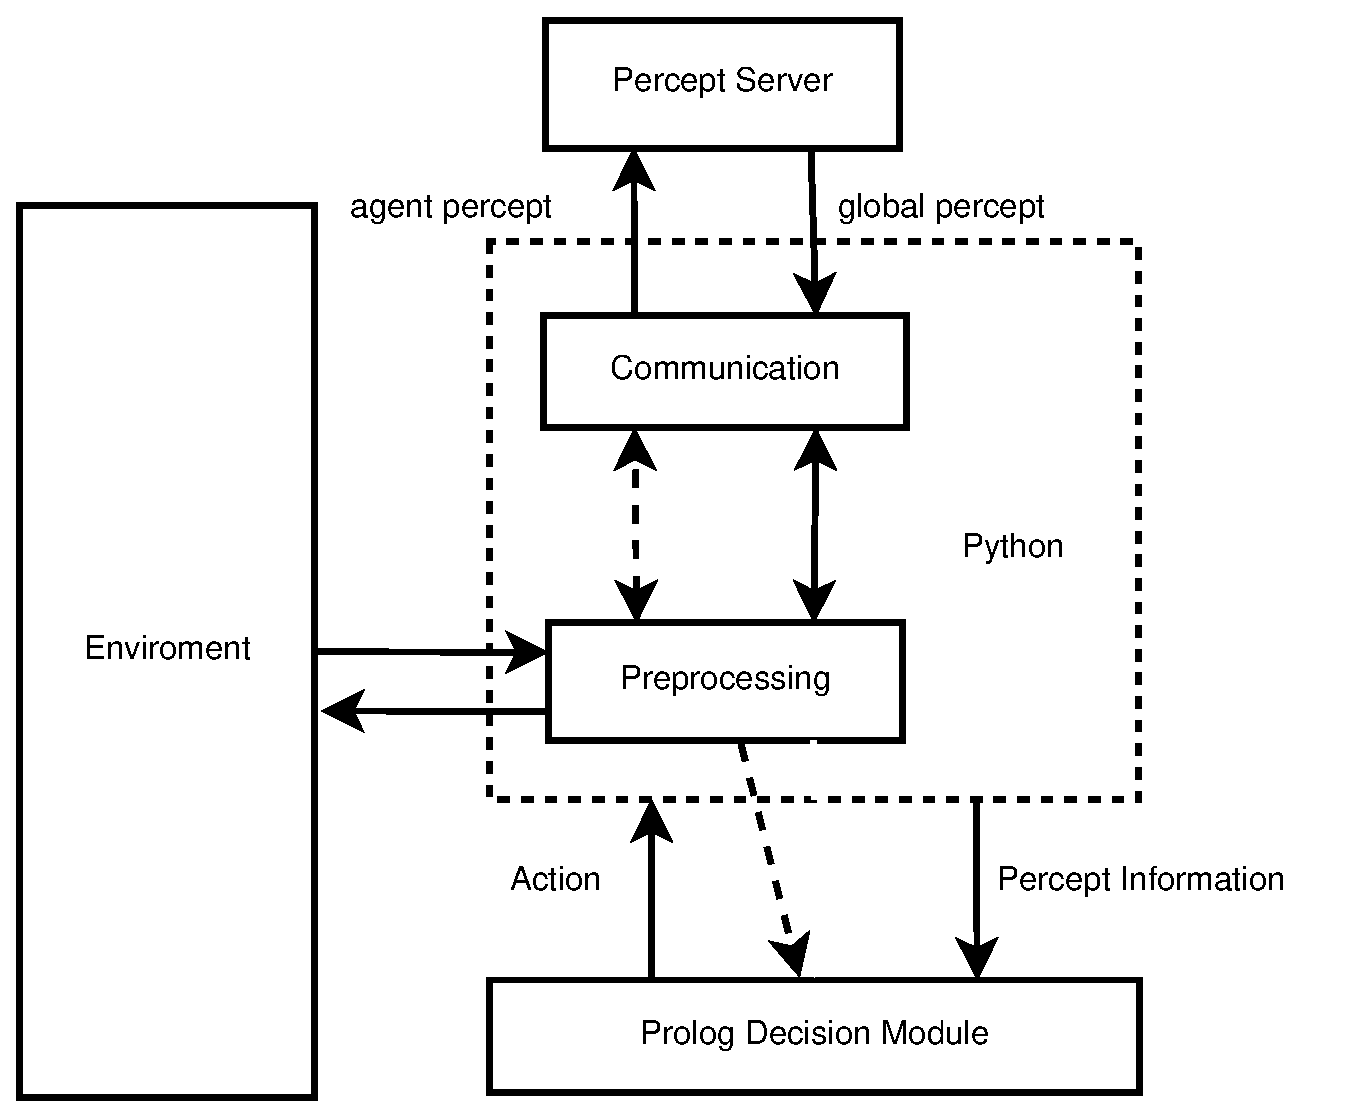
\includegraphics[scale=.5]{agent_architecture.eps}

 \caption{Diagrama de la arquitectura del agente. Las líneas punteadas representan el 
 flujo de control, y las líneas contínuas representan el flujo de datos.}
 \label{fig:architecture}
\end{figure}

El servidor de percepciones (SP) es un programa independiente, encargado de unificar las 
percepciones de todos los agentes que se encuentran en ejecución. Recibe sus percepciones 
individuales y retorna a cada uno de ellos el conjunto de datos que aún no poseen, de 
manera que todos los agentes del equipo cuenten con la misma información en cuanto al estado 
del escenario.

En cada iteración de la simulación, el agente recibe un mensaje por parte del servidor 
del juego, el cual contiene la información asociada a la percepción del turno en disputa. 
Este mensaje es parseado y traducido en una estructura que permite manipular los datos 
con mayor facilidad. Los datos son divididos en dos conjuntos, uno ``público'', el cual 
es compartido con los demás agentes del equipo, y uno ``privado''. La sección pública de 
datos es compartida a través del mencionado servidor de percepciones.

El agente une entonces su propia percepción con la percepción global recibida del servidor 
de percepciones, y genera un único conjunto de datos. Esta información es incorporada a la 
base de conocimientos, estableciendo nuevas creencias para el agente.

El módulo de toma de decisiones, analizado en la sección \ref{sec:arquitecturaBDI}, es el 
que implementa el modelo \textit{BDI} respetado por el agente. Este módulo es consultado en cada 
iteración para obtener la próxima acción a ser ejecutada. Una vez que el flujo de control 
retorna al programa principal, la acción seleccionada es enviada al servidor del juego.

\subsection{Base de conocimiento}

%\label{sec:baseConocimiento}

Como fue mencionado, la percepción del agente en cada iteración es convertida a una 
estructura de datos que permite, de manera más sencilla, manipular y compartir la 
información. Cuando el agente cuenta con todos los datos relativos a las percepciones 
del equipo, la base de conocimiento puede ser actualizada convenientemente. Una colección 
de predicados de Prolog consultados desde el programa principal se encarga de verificar 
que la información existente no resulte sobreescrita, y que información redundante no sea 
incorporada. 

La información que constituye conocimiento certero sobre el estado del escenario es 
almacenada mediante términos, que sirven como argumentos del predicado \texttt{k/1} 
(\textit{knowledge}). Cada uno de los datos de interés es representado mediante un 
término diferente. 
En muchos casos, esta clase de términos incluyen un argumento ligado al número de turno 
en el cual el dato fue percibido. De esta forma, es posible realizar ciertos análisis, 
como por ejemplo, considerar obsoleta la información de una determinada antigüedad.

	% En castellano para mantener el idioma y porque las b() 
	% están así.
\vspace*{1em}
\noindent\lit{k(equipoAgente(Agente, Equipo)).}\\
\lit{k(valorNodo(Nodo, Valor)).}\\
\lit{k(arco(Nodo1, Nodo2, Costo)).}\\
\lit{k(posicionAgente(Agente, Turno, Posici\acute{o}n)).}\\
\lit{k(equipoNodo(Turno, Nodo, Due\tilde{n}o)).}\\


Las creencias que provienen de inferencias y cálculos realizados a partir de información 
ya existente también son almacenadas mediante términos, en este caso argumentos del 
predicado \texttt{b/1} (\textit{beliefs}). Este tipo de creencias es empleado directamente 
por el módulo encargado de la toma de decisiones, y se mantienen vigentes sólo durante el 
turno en el cual fueron generadas. Es decir, que, al finalizar cada turno, son descartadas 
para evitar futuros problemas o inconcistencias.

\vspace*{1em}
\noindent\lit{b(estoyEnLaFrontera).}\\
\lit{b(posibleExplorar(Nodo)).}\\
\lit{b(haySaboteador(Nodo)).}\\


Existe cierta información que es formulada de manera hipotética. Se trata de datos 
surgidos de suposiciones realizadas sobre posibles estados futuros del escenario, a partir 
de su estado actual. Este tipo de datos resulta fundamental para facilitar los cálculos 
realizados por los algoritmos que se encargan de buscar formas de maximizar el puntaje 
del equipo. Dado que no constituye información real, sino posible a futuro, se almacena 
mediante argumentos de un predicado especial, \texttt{h/1} (\textit{hypothetical}).

\vspace*{1em}
\noindent\lit{h(nodoEquipo(Nodo, Due\tilde{n}o)).}\\
\lit{h(posicion(Turno, Agente, Nodo)).}\\


Las intenciones surgen del proceso argumentativo explicado más adelante, y son 
representadas utilizando términos. Si la intención no posee argumentos, entonces es 
representada mediante un átomo. En otro caso, se emplea un functor que denota el 
nombre de la intención, acompañado por un argumento. Las acciones, por el contrario, 
son representadas a través de listas. El primer elemento de la lista es un atómo denotando 
el tipo de acción. Y el resto de la lista contiene, ocacionalmente, un término que 
indica el argumento de la acción, como por ejemplo el nombre de un nodo o un agente.
Los planes son representados mediante listas de acciones, es decir, listas de listas.

Contrario a lo que ocurre con las creencias, tanto las intenciones como los planes 
constituyen información que debe perdurar en la base de conocimiento tantos turnos 
como sea necesario. Para este tipo de datos se emplean hechos específicos que cuentan 
con un único argumento.

\vspace*{1em}
\noindent\lit{intenci\acute{o}n(explorar(vertex7)).}\\
\lit{plan([[recharge], [goto, vertex7], [survey]]).}

\section{Arquitectura BDI} %CAMBIAR: Toma de decisiones?

\label{sec:arquitecturaBDI}

El módulo de \textbf{Toma de Decisiones} es consultado por el programa 
principal, obtiene la próxima acción a ser ejecutada, y la retorna para que 
pueda ser enviada. Esta es una secuencia que se reitera en cada uno de los 
turnos de la simulación, con la característica de que cuando es necesario 
plantear y planificar una nueva meta, intervienen una serie de componentes 
especiales, que difieren de aquellos involucrados cuando se cuenta con una 
meta ya planificada. 

En la Fig.\ref{fig:agentProlog} se pueden observar las diferentes partes de la
arquitectura interna de este módulo, sus interacciones el exterior (el 
\textbf{Módulo principal}), y sus interacciones internas con sus componentes,
tanto bases de datos como sub-módulos. Cada uno de estos componentes es 
descrito en esta sección.

\begin{figure}
% \includegraphics[width = 1.2 \textwidth]{agentprolog.eps}
 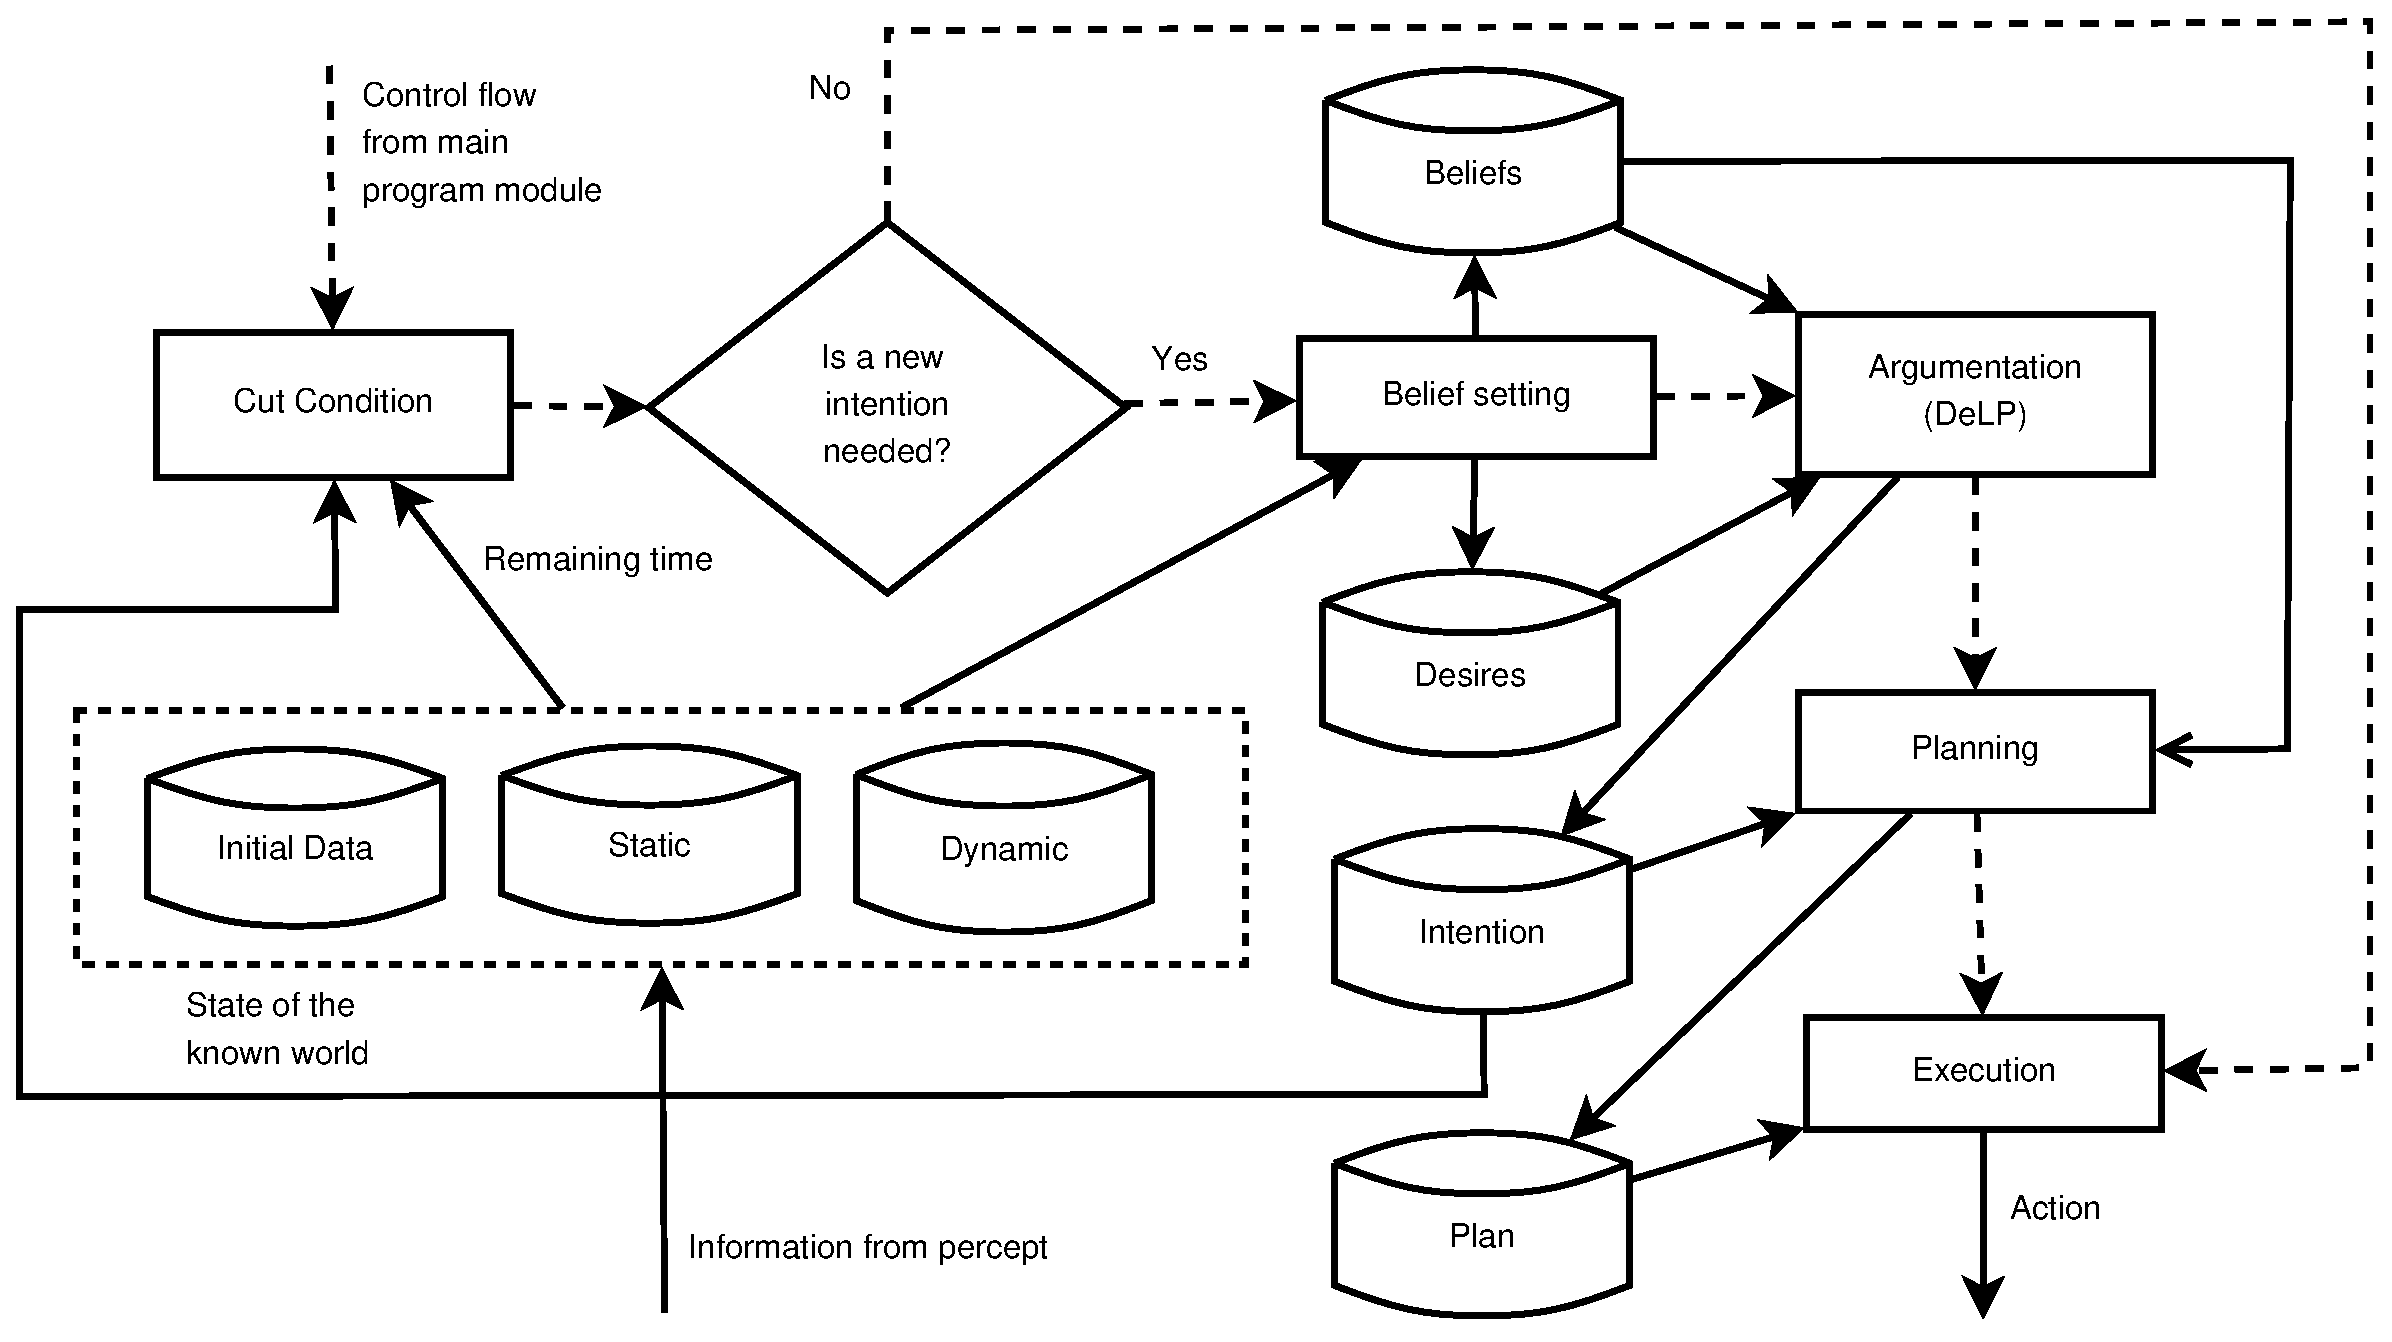
\includegraphics[width=\textwidth]{agent_prolog.eps}
 \caption{Diagrama de la arquitectura del módulo de \textbf{Toma de Decisiones}.}
 \label{fig:agentProlog}
\end{figure}

\subsection{Seteo de creencias}

\label{sec:seteoCreencias}

El seteo de creencias es llevado a cabo cada vez que el agente se dispone a 
seleccionar una nueva intención. Incluye la generación de aquellos datos que pueden 
permitir al agente realizar una elección lo más acertada posible. Se trata de 
inferencias realizadas en base al estado del escenario, es decir, aquella información 
que, como fue mencionado, es almacenada en \texttt{b/1}. No forma parte de este proceso 
la información proveniente de la percepción, las cuales denominaremos \textbf{creencias
simples}, ya que el estado del entorno es actualizado 
en cada turno de manera previa. 

\paragraph{Creencias generales.}

Existe un conjunto de creencias que resultan de utilidad general para todo el proceso 
de decisión. Entre los datos incluidos, se encuentra el puntaje que están 
aportando las zonas armadas, la diferencia de puntos que puede producirse si el agente 
abandona su posición, y la seguridad que brindan las distintas ubicaciones posibles en 
cuanto a la presencia de agentes saboteadores enemigos. 

\paragraph{Deseos.}

El proceso de toma de decisión conlleva el 
pesaje de todos los posibles deseos del agente, y la posterior selección del más beneficioso. 
Dichos deseos surgen de un conjunto predefinido, y pueden, según sea el caso, estar 
instanciados con diferentes entidades del juego, como agentes o nodos. Para que esta 
selección sea posible, es necesario determinar, de manera previa, qué deseos e instanciaciones 
son realmente factibles, y por lo tanto deben ser tenidos en cuenta, y cuales pueden ser 
descartados anticipadamente.
Para esto se analizan distintas condiciones como, por ejemplo, la distancia a un nodo 
que no ha sido explorado. Si el nodo se encuentra a una distancia que supera una cota 
pre-establecida, entonces el deseo de explorar ese nodo no es contemplado.
Los deseos e instanciaciones considerados factibles son seteados en la base de conocimiento.

\paragraph{Creencias específicas.} % Seteo de beliefs para cada deseo.

Junto con los deseos a ser evaluados, es necesario incluir en la base de conocimiento 
un conjunto de creencias relacionadas a estos deseos. Entre las más importantes, se 
encuentran las distancias que existen desde la posición actual del agente a los distintos 
vértices de interés, y la diferencia de puntaje que se produce en caso que el agente se desplace 
a dichas ubicaciones. Estos datos resultan fundamentales, ya que afectan directamente la 
valuación que se realiza de cada deseo, y por lo tanto la posterior selección. 
En esta etapa, también se produce el seteo de datos requeridos posteriormente, como son 
los caminos a los diferentes vértices analizados. 

\paragraph{Creencias defensivas.} % Seteo de beliefs en caso de agente deshabilitado.

Cuando el agente se encuentra en una situación de peligro, esto es, no posee el rol de 
saboteador y hay un saboteador enemigo en su posición, o fue atacado en el turno anterior, 
el conjunto de creencias seteadas se reduce. En estos casos, sólo son tenidos en cuenta 
los nodos vecinos, dado que representan las vías de escape más rápidas; son calculadas 
las distancias a estos (en cantidad de turnos), y las diferencias de puntaje que produciría 
el desplazamiento del agente. Esto tiene el objetivo de minimizar la cantidad de deseos 
considerados: sólo son evaluadas la posibilidad de permanecer en la misma ubicación 
(si el beneficio en puntaje es considerable), y las distintas alternativas de defensa 
propia que pueden llevar al agente a superar el peligro.

\subsection{Argumentación}

\label{sec:argumentacion}

Una vez finalizado el seteo de creencias, el agente procede a la selección de la próxima 
intención. Para esto, se toma cada uno de los deseos marcados como factibles en la base 
de conocimiento, y se consulta al módulo de argumentación \cite{Amgoud:2008}\cite{Rotstein:2007}(implementado en \DLP\cite{Ferretti:2008}) sobre éstos. 
Dicho módulo
%considera que existen razones para creer realizables sólo aquellos deseos que satisfacen 
%sus condiciones. 
devuelve como garantizados los deseos que son realizables, es decir aquellos que satisfacen
una serie de condiciones.
Para éstos, obtiene un valor que representa su peso, en términos del 
beneficio que conllevan para el equipo. El deseo que presenta el mayor peso entre los 
analizados, se convierte en la nueva intención del agente, la cual es almacenada hasta ser 
alcanzada o reemplazada.

Tanto la evaluación como el pesaje de los deseos, son llevados a cabo empleando \textit{argumentación} 
en un módulo especial, implementado con la ayuda de \DLP. 
Detalles sobre la implementación y como la argumentación es aplicada en el proceso de 
razonamiento, son estudiados en el capítulo dedicado a la Toma de Decisiones. %referencia, cambiar nombre?

\subsection{Planificación}

%\label{sec:planificacion}

La planificación consiste en obtener la secuencia de acciones que llevan al cumplimiento 
de la intención propuesta. Esta lista está compuesta por las acciones que le permiten al 
agente posicionarse en el nodo deseado, y, en algunos casos, una acción concreta a realizar. 
Como se dijo anteriormente, en la etapa de seteo de creencias, todos los caminos hallados 
por el algoritmo de búsqueda son almacenados. Dicho algoritmo fue implementado de manera 
tal que los caminos no están constituidos por nodos o vértices, sino por una secuencia 
optimal de acciones, que tiene en cuenta no sólo el nodo destino, sino también los recursos 
del agente, y la meta final a realizar (en caso de haber una acción final). De esta forma, 
cualquiera haya sido la intención elegida, el agente cuenta en su base de conocimiento 
con el plan necesario para cumplirla. La planificación se resume entonces a tomar las 
acciones correspondientes, y establecerlas efectivamente como el plan a seguir.

Alternativamente, esta etapa puede introducir ciertas acciones con el objetivo de optimizar 
el uso del turno. En aquellas situaciones en que el agente se dispone a permanecer inactivo, 
la acción nula (\texttt{skip}) puede ser reemplazada por la acción de recargar energía, si es que 
esta resulta más productiva.

\subsection{Ejecución}

\label{sec:ejecucion}

Dado que el plan se encuentra almacenado de manera completa y ordenada, la ejecución se 
realiza en forma directa. Se toma la próxima acción, es decir, la primera acción del plan 
restante, y se la retorna al módulo principal del programa. Este se encarga posteriormente 
de enviarla al entorno, para que se convierta finalmente en la siguiente acción realizada 
por el agente.

\subsection{Condición de corte}

\label{sec:condicionDeCorte}

Existen situaciones en las que el paso de los turnos genera que el cumplimiento de una 
meta se vuelva inalcanzable, innecesario, riesgoso, o menos productivo de lo previsto, por 
lo que resulta más beneficioso abortar el plan existente, y seleccionar una nueva intención. 
Ésta es una etapa de verificación, que tiene como objetivo la detección de este tipo de 
situaciones. Es ejecutada sólo en aquellos turnos en los que el agente se encuentra 
siguiendo el plan de una intención previamente determinada.

Cada deseo o esquema de deseo cuenta con una serie de \textbf{condiciones de corte}, que 
son evaluadas al inicio de cada turno, en caso de existir un plan establecido. Si se verifica 
que alguna de estas condiciones se satisface, entonces la intención es descartada, y el 
agente ingresa en un nuevo proceso de selección. 
Entre las condiciones de corte tenidas en cuenta, se encuentran: 

\begin{itemize}
	\item Que haya pasado una determinada cantidad de turnos desde el inicio del plan.
	\item Que el agente se encuentre deshabilitado.
	\item Que haya sido atacado o se encuentre amenazado por un enemigo.
	\item Que la meta haya sido alcanzada por un compañero de equipo.
\end{itemize}

\subsection{Re-planificación}

La fase de re-planificación consiste en elaborar nuevamente el plan que permite alcanzar 
la meta propuesta, sin modificar dicha meta. Este paso, como el anterior, se realiza en 
los turnos en los que el agente posee un plan pre-calculado. Dado que en estos turnos no 
es necesaria la obtención de una nueva intención, proceso que implica el mayor insumo de 
tiempo, la inclusión de la re-planificación no afecta el funcionamiento normal del agente, 
en términos de tiempo de ejecución. 

Por el contrario, existe una mejora en el desempeño del equipo, surgida de un mejor 
aprovechamiento de la información percibida. Los agentes actualizan su información sobre 
el estado del mundo en cada turno. Datos como el estado en que se hallan los recursos del 
agente, la incorporación de nodos y arcos hasta el momento desconocidos, o las nuevas 
ubicaciones de los otros agentes, permiten elaborar planes más precisos y ajustados a la 
realidad que los originalmente diseñados. Así, los agentes son capaces de cumplir sus 
metas con mayor facilidad, o abortarlas si es necesario.

%%%%%%%%%%%%%%%%%%%%%%%%%%%%%%%%%%%%%%%%%%%%
%%%%%%%%%%%%%%%%%%%%%%%%%%%%%%%%%%%%%%%%%%%%


\chapter{Argumentación}

En esta sección se expandirá lo explicado en el capítulo anterior, relacionado a 
la toma de decisiones. Esto es, generación de los deseos, su estructura, la selección de la
intención, en particular su proceso de argumentación (derrotas, tanto por peso como 
propias), todo con ejemplos concretos del programa realizado. 

\section{Modelo de argumentación} 

\label{sec:modeloDeArgumentacion}

Sin inmiscuirse en los detalles de la implementación, la idea que llevamos a cabo en el 
desarrollo del programa fue un sistema en el que existen un tipo especial de argumentos,
que constituyen los argumentos de deseos, los cuales contienen un valor numérico.
Este valor es el \textbf{peso} del deseo que es garantizado por el argumento de deseo. 

El soporte de cada argumento de deseo, está formado por reglas rebatibles que representan
razones para considerar la aplicación del deseo beneficiosa para el agente y/o el equipo.
A su vez, estos argumentos requieren de la existencia de distintos hechos en la base de 
datos consistente, para estar garantizados. Se trata de creencias, algunas de las cuales
contienen cuantificaciones acerca del estado del mundo actual (por 
ejemplo, el valor de un nodo o el costo de un arco). Estos valores son utilizados en la
determinación del peso del deseo aplicando un cálculo \textit{ad hoc}, %cursiva
que será explicada luego.

Dado que sólo resultará seleccionado un único deseo, se contraponen todos los argumentos 
de deseo garantizados, generando ataques entre sí. Entre dos argumentos enfrentados, será
derrotado el de menor peso. Por lo tanto, quedará como no derrotado un solo argumento, 
aquel con el mayor peso. Estos ataques, en \DLP, pueden ser programados de la 
siguiente manera:

\nlA{\srule{\no X}{Y}}

Siendo $X$ e $Y$ cualquier deseo. Este tipo de reglas estrictas, a las que
denominaremos \textit{reglas de cancelación mutua}, se repite para todos los 
deseos existentes.

Entre los criterios de comparación comunes de \DLP\ (estos son \textit{Especificidad} y 
\textit{Derrotadores a asunciones}) no existe la capacidad de comparar por pesos. 
Por esta razón, se utiliza un nuevo criterio, el cual 
denominaremos \textit{Mayor Peso}. Como su nombre lo indica, compara los pesos de los 
argumentos, si estos existen (y estos sólo existen en los argumentos de deseos). Los 
argumentos con mayor peso derrotan a los de menor.

En el caso de que el peso de dos argumentos sea el mismo, todavía existiría el problema 
de los bloqueos. Esto generaría un problema si justo se tratará de los más pesados, ya 
que ninguno de los dos (o más) deseos estarían garantizados o derrotados, y la consulta
por deseo no devolvería ningún resultado. Por esta razón, se extiende el criterio 
\textit{Mayor Peso}\ para que contemple como caso especial las igualdades de peso. En 
estos casos, se hará una comparación por orden lexicográfico de los argumentos, ya que
no interesa cuál de los dos resulta ganador. 

\begin{figure}
% \includegraphics[width = 1.2 \textwidth]{agentprolog.eps}
 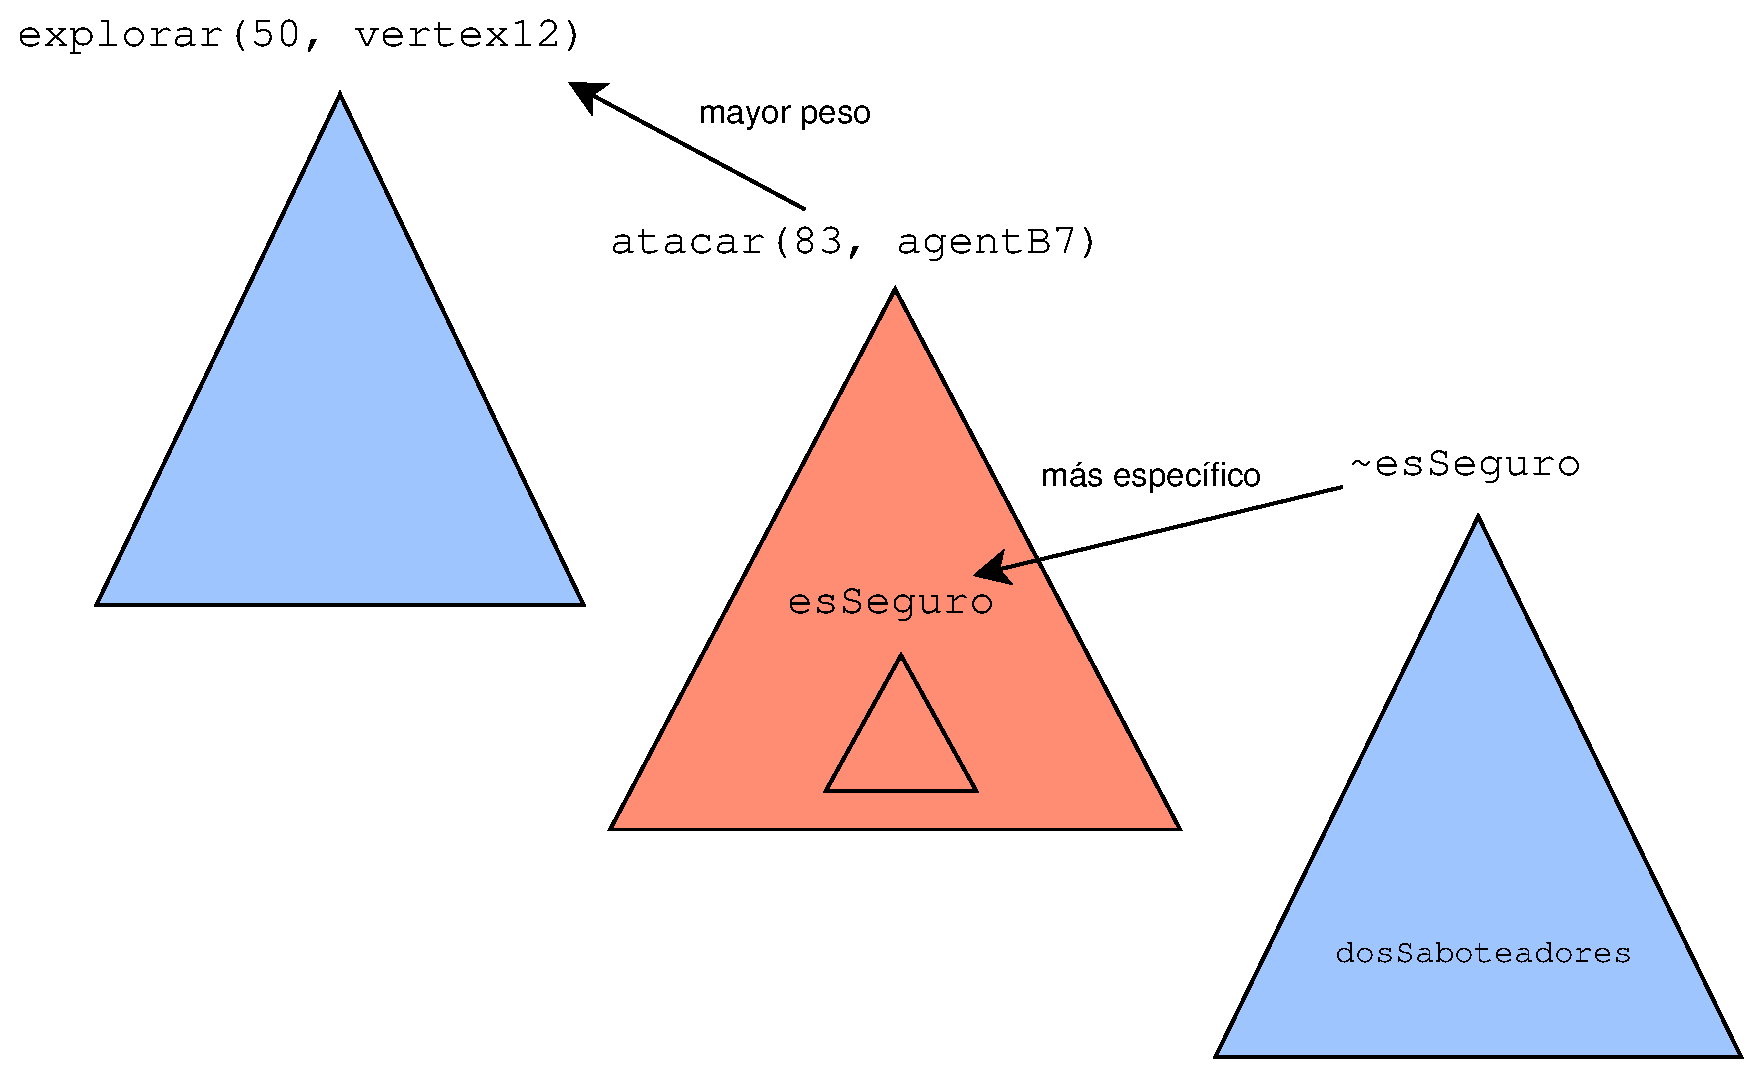
\includegraphics[width=\textwidth]{mamarracho.eps}
 \caption{Ejemplo de un árbol dialéctico posible dentro del modelo explicado.}
 \label{fig:mamarracho}
\end{figure}

En la figura \ref{fig:mamarracho} se muestra un ejemplo hipotético de este 
concepto de derrotas. Se 
trata de un árbol dialéctico con tres argumentos, de los cuales dos son
argumentos de deseos, \textbf{explorar} y \textbf{atacar}. El primero es
derrotado por el segundo, por el criterio de comparación \textit{mayor peso},
ya que el peso de \textbf{atacar} es de 83, lo cual representa que hay más 
razones para realizarlo que el deseo de \textbf{explorar}, con peso de 50. Sin
embargo, \textbf{atacar} tiene como subargumento la asunción de que el deseo es
seguro, lo cual es incongruente con el argumento de que no es seguro, el cual 
es más específico, ya que se basa en más razones para asegurar su veracidad 
(como la creencia \texttt{dosSaboteadores} fue asertada, el agente tiene 
razones para considerar al deseo de atacar como inseguro, ya que puede verse
en desventaja numérica frente a dos saboteadores enemigos).

Al realizar el marcado de este árbol, el argumento de deseo que queda 
garantizado es el de \textbf{explorar}, por lo cual este deseo sera el devuelto
como intención. En la figura, ésto es representado por los colores azul (para
\textit{undefeated}) y rojo (para \textit{defeated}).


\section{Tipos de argumento}

\label{sec:tiposArgumento}

% En el subprograma de toma de decisiones (a partir de ahora subprograma \textit{DeLP}, o simplemente
% \textit{DeLP}), se utilizaron dos tipos de argumentos. En esta sección, se explicará su uso.

El esquema anterior fue el propuesto, pero no exactamente el implementado, ya que
realizamos modificaciones para optimizar los tiempos de ejecución del programa. Sin 
embargo, el concepto de tener varios tipos de argumentos, incluyendo el de deseos, con sus
pesos, se mantuvo. En esta sección se explicarán más en detalle.

\subsection{Argumentos de Creencias}

\label{sec:argumentosSoporte}

\begin{definicion}
	Un \textit{argumento de creencia} es un argumento cuya conclusión denota una creencia 
	sobre el estado del mundo.
\end{definicion}

Los argumentos de creencias pueden actuar como subargumentos de los argumentos
de deseo, así como también convertirse en derrotadores de estos mediante ataques a 
subargumentos. No incluyen peso, aunque pueden contener los valores que serán utilizados 
para calcular éstos, entre otros usos. En la Fig. \ref{fig:mamarracho}, \lit{esSeguro}, 
\lit{\no esSeguro} y \lit{dosSaboteadores} constituyen argumentos de creencias.

\subsubsection{Creencias Generadas}

Este conjunto es asertada en el seteo de creencias, como fue explicado en %REFFFFFFF
. Se trata de hechos \DLP, cuya cabeza contiene la signatura encerrada dentro
de un functor \texttt{b/1}. Esto se hizo para facilitar la búsqueda y eliminación de
estos hechos. Un ejemplo de éstos sería el siguiente hecho:

\nlA{b(\no esSeguro(vertex34)).}

Este hecho determina que en el turno actual, la posición \texttt{vertex34} es peligrosa,
ya que se encuentra un saboteador enemigo parado en él. Varios deseos tienen en cuenta
que la posición a la que irán sea segura, ya que sino entrarían en un posible combate.
Luego, un deseo que necesite tener como parámetro un vértice seguro, lo descartaría.

La existencia o no de estos hechos corresponde con una semántica binaria. Otros tipos de
creencias en el subprograma \DLP\ no se corresponden con ella, a pesar de corresponderse
con el esquema anterior. Se trata de creencias que exponen cuantificaciones a ser 
tenidas en cuenta para el cálculo de los pesos. Un ejemplo de estas creecias es el 
siguiente:

\nlA{b(difPuntosSinMi(0)).}

En este caso, el hecho expone la cantidad de puntos que se podrían llegar a perder si el
agente se va de su vértice (ya sea porque se mueve o porque deja de estar activado). Esa
cantidad se tiene en cuenta por los argumentos de deseos, para descartar los que generen
mucha pérdida de puntos. \textit{``Mucha pérdida''} se corresponde con un 
concepto difuso, a diferencia de los hechos explicados antes. Este valor será 
el parámetro de una función de varias variables, que será explicado luego, el 
cual genera el valor que se usa como peso del argumento de deseo. Perder cero 
puntos, como expone el hecho de más arriba, es el caso ideal de un deseo, por 
lo que las metas que lo consideren tendrán un puntaje relativamente alto.

Existen otras creencias de este tipo, que pueden tener otros parámetros además del valor
numerico, como por ejemplo un vértice. El hecho \texttt{difPuntos} es un ejemplo de esto.
Es parecido al anterior, con la diferencia que se instancia con un vértice al cual es
posible llegar en una cantidad pequeña de turnos, y su otro parámetro representa la
cantidad de puntos que ganaría (o perdería, si el valor es negativo) el agente al moverse
a dicho vértice. Por esta razón, puede haber varias de estos hechos instanciados con
distintos vértices la vez.

\subsubsection{Creencias indirectas}

\label{sec:creeciasIndirectas}

Hay algunas creencias que no se generan en tiempo de ejecución del programa Prolog, sino
que se calculan cuando se ejecuta el subprograma \DLP. Se calculan en base a las creencias
expuestas en la sección anterior. Un ejemplo de éstas es la de la Fig. 
\ref{fig:creenciaIndirecta}.

\begin{figure}[h]

\nlA{\drule{puedoHacerParry}{myRole(repairer)}}
\nlA{\drule{puedoHacerParry}{myRole(saboteur)}}
\nlA{\drule{puedoHacerParry}{myRole(sentinel)}}
\nlA{\drule{\no puedoHacerParry}{myEnergy(Energy), less(Energy,2)}}


\caption{Ejemplo de una creencia indirecta.}
\label{fig:creenciaIndirecta}

\end{figure}

En este caso, la creencia \lit{puedoHacerParry}\ se calcula en base al rol del 
agente,
así como también de la energía del agente. Esto es porque no todos los roles tienen la
acción asociada, por lo que se listan las que sí lo pueden. Por otro lado, el agente
no puede hacer \textit{parry}\ si no tiene por lo menos dos puntos de energía, lo cual
es expresado por la última regla.

\subsubsection{Funciones aritméticas y lógicas}

En la última línea de la Fig. \ref{fig:creenciaIndirecta}, se utiliza la función 
\texttt{less/2}, que es una función de comparación. (En ese caso, devuelve lo mismo
que $Energy < 2$.) Ése es un ejemplo de las diferentes funciones aritméticas y 
lógicas que se encuentran en el subprograma \DLP.

Estas reglas se encuentran fuera del lenguaje \DLP, y fueron implementadas 
aprovechando su capacidad de consultar a Prolog, utilizando \textit{built in's}.
En la figura \ref{fig:funciones}\ se ejemplifica la manera en que se han 
implementado.

\begin{figure}[h]
\begin{Verbatim}[numbers=left]
is_a_built_in(less(_X,_Y)).
is_a_built_in(add(_X,_Y,_Z)).

add(X,Y,Z :- Z is X + Y.
less(X,Y) :- X < Y.
\end{Verbatim}

\caption{Implementación de una función aritmética y una lógica.}
\label{fig:funciones}
\end{figure}

\subsubsection{Coeficientes y otros valores auxiliares}

En la fórmula de la figura \ref{fig:calculoDePeso}\ se utiliza el valor 
\texttt{CoefFase}. Este valor no pertenece a lo obtenido en las percepciones, ni
directa ni indirectamente, sino que se trata de un valor preestablecido (o
\textit{harcodeado}). Pertenece a esta categoría aparte de creencias predefinidas,
cuyos valores modifican los pesos ya sea de manera aditiva/substractiva, o 
porcentualmente (como es el caso de \texttt{CoefFase}).

En particular, este valor se refiere a un coeficiente que se le aplica a varios
pesos de deseos, que representa la utilidad de cada deseo en la fase actual. El 
concepto de \textit{``fase''}\ se trata de un modificador más del comportamiento
del agente, que cambia de acuerdo a diferentes parámetros, como por ejemplo una
determinada cantidad de turnos, proporción de muertes, porcentaje de mapa explorado,
etc. Fue implementada la interfaz para utilizarla, pero no se expandió a más de una
fase inicial de exploración, por cuestiones de falta de tiempo.

Otros valores caen dentro de esta categoría, como \lit{agentRolePoints/3}.
Se utiliza para agregar (o sustraer) una determinada cantidad de turnos, dado el
deseo y el rol del agente al cual está apuntado el deseo. Esto sirve para modificar el 
comportamiento de una manera sencilla y modular, para los deseos y roles que los 
necesiten.

Se necesitarían $|{\mathcal D}| \times |{\mathcal R}|$ reglas para determinar 
estos valores, siendo $\mathcal D$ y $\mathcal R$ los conjuntos de deseos y 
roles respectivamente. Ésto se simplificó utilizando un valor por defecto 
neutral ($0$). Este comportamiento es mostrado en la Fig. 
\ref{fig:agentRolePoints}. En éste se muestra la implementación del caso 
general, y el caso especial del deseo \emph{reparar}\ para el rol 
\emph{repairer}. Agregarle 70 puntos al peso implica darle mayor importancia 
reparar a otro reparador, antes que hacerlo con cualquier otro agente.

\begin{figure}[h]
\begin{Verbatim}[numbers=left]
% en arg.delp
agentRolePoints(_, _, 0) -< true.
	
~agentRolePoints(D, R, 0) <- 
	agentRolePoints(D, R, V),
	notEqual(V, 0).
    
% en repairer.delp
agentRolePoints(reparar, repairer, 70) <- true.
\end{Verbatim}
\caption{Implementación de \lit{agentRolePoints/3}, para el caso general, y para el 
deseo de \emph{reparar}\ para el \emph{repairer}.}
\label{fig:agentRolePoints}
\end{figure}


\subsubsection{Cálculo de pesos}

Utilizando la misma idea que la funciones ariméticas de la sección anterior, el
cálculo de los pesos de los argumentos de deseos se logró utilizando \textit{built 
in's}. Existe uno por cada regla de deseo, salvo que esté fijo, en cuyo caso 
este valor simplemente se encontrará en vez de la varialbe \texttt{Peso}. Un 
ejemplo extraído del código se encuentra en la Fig. \ref{fig:calculoDePeso}.

\begin{figure}[b]
\begin{Verbatim}[numbers=left]
is_a_built_in(aumentoPeso(_, _, _, _, _)).

aumentoPeso(Turnos, DifPuntos, EnergiaRestante, CoefFase, Peso) :-
    Peso is (DifPuntos * 10 + (10 - Turnos) ** 2 + EnergiaRestante) * 
    		CoefFase.
\end{Verbatim}
\caption{Implementación del cálculo del peso de un argumento de deseo.}
\label{fig:calculoDePeso}
\end{figure}

%En este ejemplo, se calcula el peso del deseo \emph{aumento}. Para esto, se utilizan
%varios parámetros, entre las cuales se encuentran la cantidad de turnos que 
%conllevará realizarlo, y la diferencia de puntos que genera.

Todas estas funciones cumplen con el protocolo de mantener el nombre del deseo,
seguido de ``Peso'' como nombre. A su vez, mantiene todos los parámetros 
necesarios como argumentos, seguido de la variable \texttt{Peso}, en la cual se 
retornará dicho valor.

El proceso de la definición de las fórmulas utilizadas para este cálculo fue 
realizado de manera \textit{ad hoc}, a partir de la prueba y error. Se trató
de balancear todos las fórmulas de manera tal de que los valores promedio 
estuvieran alrededor de 100, los bajos por debajo de 20 (sin necesidad de ser
mayores a 0), y los más altos alrededor de 500. Existen fórmulas para esquemas
de deseos de alta prioridad que tienen pesos que pueden superar 1000.

En general, se realiza la suma de los parámetros, modificados de alguna manera.
Se agrupan valores que aportan al deseo de manera lineal, y de manera cuadrática
(esto es, interesa más el orden de magnitud del valor que el valor en sí), los
cuales sumarán o restarán dependiendo de su aporte al deseo. A su vez, 
existirán coeficientes que modificarán todo el valor calculado.

En el ejemplo de la Fig. \ref{fig:calculoDePeso}, se puede observar la fórmula 
utilizada para el cálculo del peso del deseo \textit{Aumento}:

$$(10 \times DifPuntos+ (10 - Turnos) ^ 2 + EnergiaRestante) \times CoefFase$$

El valor de la cantidad de puntos que el agente obtiene por realizar este deseo
es central si se desea aumentar la zona, por lo que el valor está multiplicado
por 10. Se priorizarán los deseos que tengan los planes más cortos, por lo cual
se suma un valor que aumente cuadráticamente cuando los turnos disminuyan. Los 
planes nunca superarán los 10 turnos (ésto es controlado en el seteo de 
creencias), por lo que no se corre peligro de que aumente involuntariamente.
La energía restante es un valor pequeño, ya que la energía máxima ronda los 12
puntos. Se suma este valor para desempatar casos en los que haya dos deseos 
del mismo esquema con distinto plan que tengan puntajes cercanos. Finalmente,
se multiplica todo por el coeficiente de la fase, el cual si no está definido 
será 1.


\subsection{Argumentos de Deseos}

\label{sec:argumentosDeseos}

En esta sección, se darán las diferentes definiciones que se utilizarán para dar marco a los
argumentos de deseos, que son los argumentos que modelan el comportamiento de los agentes.

\begin{definicion}
	Un \textbf{esquema de deseo}\ es un literal no negado, y tiene por lo menos 
	un parámetro. Estos parámetros no deben estar instanciados.
\end{definicion}


El nombre del functor del esquema de deseo connota el deseo que se quiere 
representar. Un ejemplo para ésto sería:

\nlA{\lit{explorar(Peso, Vertice)}}

Este esquema de deseo es el utilizado en la Fig. \ref{fig:mamarracho}, que a 
su vez es un ejemplo extraído del programa. Las siguientes definiciones también
tendrán ejemplos basados en \textit{explorar}.

\begin{definicion}
	Un \textbf{deseo} es un esquema de deseo con sus parámetros instanciados.
\end{definicion}

La interfaz con Prolog consultará por estos deseos al programa \DLP, de los 
cuales seleccionará al mejor como \emph{intención}. El primer parámetro 
siempre corresponderá al peso del deseo. Los otros parámetros contienen 
información relacionada, como por ejemplo el vértice o un agente al cual hace 
referencia, y son los necesarios y suficientes para determinar unívocamente al
deseo. Esto es, no existen dependencias funcionales (en el sentido de 
\emph{base de datos}) entre los parámetros. Un ejemplo de deseo seria:

\nlA{\lit{explorar(50, vertex12)}}

Este deseo es el que queda garantizado en la Fig. \ref{fig:mamarracho}. Su 
objetivo es que el agente se traslade al vértice 12 para 
realizar un reconocimiento (la acción \texttt{survey}) del terreno en dicho
lugar. Su peso es de 50, y fue calculado en base a varios valores relacionados
a este objetivo, como la distancia al vértice, o la cantidad de puntos de zona
que el equipo gana o pierde con dicho movimiento.


\begin{definicion}
Una {regla de deseo} es una regla rebatible o una regla estricta cuya cabeza es un esquema 
de deseo.
\end{definicion}

El programa \DLP\ está conformado por una serie de reglas de deseo, que modelan
el comportamiento del agente, así como de otras reglas que serán utilizadas por los 
argumentos de creencias. Un ejemplo de una de estas reglas es el de la Fig. 
\ref{fig:deseoExplorar}.

\begin{figure}[h]
\begin{equation*}
\begin{aligned}
explorar&(Peso, X)\; \defleftarrow \;\\
	&b(distancia(X, [[survey]], Dist, EnergiaRestante)),\\
    &greaterEq(Dist, 3),\\
    &b(difPuntosSinMi(DifPuntos)),\\
    &positivoONegativo(DifPuntos, Positivo, Negativo),\\
    &phaseCoef(explorar, Coef),\\
    &explorarValue(Dist, Positivo, Negativo, EnergiaRestante, \\
    &Coef, Value).
\end{aligned}
\end{equation*}
\caption{Una de las reglas del deseo \emph{Explorar}}
\label{fig:deseoExplorar}
\end{figure}

Como fue explicado en la sección \ref{sec:modeloDeArgumentacion}, el tipo más importante de 
argumentos en el subprograma \DLP\ son los de argumentos de deseos. 

\begin{definicion}
	Un \textbf{argumento de deseo} es un argumento cuya conclusión es un deseo.
\end{definicion}

Siguiendo la definición de argumento expuesta en la sección, un ejemplo para
\textbf{argumento de deseo} sería el que se encuentra en la Fig. 
\ref{fig:ejemploArgDeseo}.

\begin{figure}[h]

\begin{equation*}
\LEFTRIGHT\langle\rangle{
\LEFTRIGHT\{\}{
\begin{aligned}
ex&plorar(50, vertex12)\; \defleftarrow \; \\
    &b(distancia(vertex12, [[survey]], 3, 2)), \\
    &greaterEq(3, 3),\\
    &b(difPuntosSinMi(0)),\\
    &positivoONegativo(0, 0, 0),\\
    &phaseCoef(explorar, 1),\\
    &explorarValue(3, 0, 0, 2, 1, 50).
\end{aligned}
}
,\, explorar(50, vertex12) 
}
\end{equation*}



\caption{Argumento para el deseo $explorar(50, vertex12)$.}
\label{fig:ejemploArgDeseo}
\end{figure}

\section{Selección de la Intención}

El proceso de selección se realiza mediante la consulta al programa \DLP\ por cada
uno de los deseos, como se explicó en la sección \ref{sec:argumentacion}. 
En esta sección se detalla como el modelo de argumentación planteado, fue integrado al marco
argumentativo provisto por \DLP.

\subsection{Construcción de argumentos de deseo}

La construcción de un argumento de deseo se produce cuando el programa \DLP\ es 
consultado por un deseo particular. Para esto, se busca una regla de deseo cuya cabeza sea
el modelo de deseo al que pertenece el deseo consultado. A partir de esta, se genera un 
argumento, como se introdujo en la sección %REFFFFFFF

Existen circunstancias que pueden impedir la construcción de un argumento para un determinado
deseo. En el proceso de construcción, \DLP\ puede encontrarse con la imposibilidad de generar
una derivación rebatible. Por la forma en que fue diseñado el sistema, la única posibilidad de
que esto ocurra se debe a la falta de hechos, que deberían haber sido suministrados durante el
seteo de creencias, o se trata de predicados \textit{built in} que no pueden ser generados. 

\subsubsection{Falta de creencias}

El faltante de creencias puede ser causado por dos motivos. Por un lado, puede 
deberse a la incapacidad para calcularlas. Otra causa es que, en tiempo de seteo de creencias,
se descubran razones para creer que el deseo relacionado con la creencia ha dejado de tener 
sentido, por lo cual dicha creencia no es asertada de forma deliberada, imposibilitado a \DLP\ 
para generar el argumento.

Un ejemplo claro de este comportamiento es el de la creencia de distancias. 
Se trata de la cantidad de turnos que cuesta un plan. A partir de un
deseo, se calcula un camino que culmine en el vértice al cual el agente desea ir. Puede suceder que 
este camino no exista, o sea, no sea posible generarlo a partir de la base de conocimiento del 
agente, siendo este caso el primero de los explicados más arriba. 

En la búsqueda de caminos, se podan las ramas de una determinada longitud. Esto se realiza para evitar
tiempos de ejecución excesivos, pero también porque un deseo que tenga asociado un plan con una 
longitud mayor a la determinada, deja de tener sentido. Éste comportamiento es el explicado en el 
segundo de los motivos para la falta de hechos.

\subsubsection{Condiciones insatisfechas}

Las reglas de deseos pueden tener condiciones establecidas sobre los valores relacionados al deseo,
o aserciones, que
si no son satisfechas impiden la construcción del argumento de deseo. Se trata de relaciones aritméticas,
implementadas a partir del predicado \texttt{is\_a\_built\_in}, y calculadas por demanda en Prolog.

Por ejemplo, puede ser utilizado para chequear en Prolog que un deseo de expansión a un vértice genera
algún beneficio, al condicionar a la diferencia de puntos de zona a ser positivo.

\subsection{Conflictos}

Los conflictos que puedan tener los argumentos de deseo pueden ser los típicos de \DLP,
presentados anteriormente, o
los pertenecientes al modelo de argumentación. Estos últimos son los conflictos suscitados entre 
los argumentos de deseos entre sí, implementados en el modelo con las \textit{reglas de cancelación
mutua}. En la implementación del sistema, este comportamiento fue simulado desde Prolog, por lo que 
no fueron necesarias éstas reglas. En la sección siguiente se explicará cómo fue simulado.

\subsection{Derrotas y Garantías}

Los únicos criterios de comparación usados fueron la \textit{especificidad} y la \textit{derrotador a 
asunciones}. Para los deseos que son garantizados por \DLP\ se generan sus respectivos árboles de dialéctica, como 
fue explicado en la sección %REFFFF
No fue necesario implementar el criterio \textit{Mayor peso}, ya que este comportamiento
fue simulado por la interfaz con Prolog.

Como fue explicado, en el modelo todos los argumentos de deseos se encuentran en conflicto, y el 
único que queda como no derrotado es el de mayor peso. Para simular ésto, Prolog consulta 
secuencialmente por todos los deseos, y va manteniendo el de mayor peso. Entonces, los otros deseos
quedan derrotados de manera implícita.

%%%%%%%%%%%%%%%%%%%%%%%%%%%%%%%%%%%%%%%

\chapter{Relación con DeLPAP}

Este capítulo se mostrará DeLPAP, el cual es un lenguaje APL (Agent Programming 
Language) basado en DeLP, y siguiendo el espíritu de 3APL. Este lenguaje fue
desarrollado por el Dr. Sebastián Gottifredi en su tesis doctoral, por lo que 
aportó sus conocimientos y descubrimientos en el área, en el diseño del sistema
multi-agente. Este aporte se ve reflejado en las similitudes entre los dos 
sistemas, las cuales se mostrarán también en el transcurso del capítulo.

\section{DeLPAP}

DeLPAP es un lenguaje de programación de agentes declarativo que utiliza 
DeLP-Servers para ejecutar los programas que modelan a los agentes. Un 
DeLP-Server es una implementación \textit{standalone} de DeLP, la cual 
tiene una arquitectura de cliente-servidor. 

\subsection{DeLP-Servers}
Un DeLP-Server mantiene un programa DeLP, al cual los clientes le realizan consultas. 
Para responderlas, el DeLP-Server utilizará la información pública almacenada 
en él, en conjunto con información individual enviada por los clientes a 
través de la consulta, creando un contexto especial para ésta. Este contexto 
es conocimiento que el servidor utilizará solamente para esa consulta en particular, y no afectará consultas futuras.

\begin{definicion}[Consulta contextual]
Sea \PP\ = \SD, una consulta contextual para \PP\ es un par 
\cquery{(\addset,\remset)}{Q}, donde $Q$ es una consulta \DLP, \addset\ y 
\remset\ son un conjunto de literales no contradictorios.
\end{definicion}

Este tipo especial de consulta contextual agrega y remueve temporalmente
elementos de \PP. Los literales de \addset\ serán agregados como hechos a 
\SSet, siempre y cuando se pueda asegurar que se mantendrá la consistencia.
Los literales de \remset\ determinarán dos acciones: las reglas y hechos a ser 
removidos de \SSet, y las reglas rebatibles a ser removidas de \DD.

\subsection{Definición de DeLPAP}

En esta sección se mostrará como la argumentación rebatible puede ser 
integrada en APL utilizando DeLP-Servers. Se definirá un lenguaje de 
programación de agentes declarativo llamado DeLPAP. Este lenguaje está 
basado parcialmente en 3APL %citar
, donde las interacciones entre los componentes mentales son realizadas a
través de consultas (en el sentido de consulta a un programa lógico).
Siguiendo este modelo, se utilizarán consultas contextuales para modelar la 
interacción entre los componentes de los agentes.

\subsubsection{Sintaxis}

Los agentes en DeLPAP están caracterizados por tres componentes: creencias,
metas y un conjunto de esquemas de planes. % TODO: ver si esta traducción es correcta
Éstos representan los componentes del estado
mental del agente, y serán especificados por programas \DLP, las cuales
serán usadas para computar las creencias y las metas en cada ciclo 
deliberativo. Los esquemas de planes serán usados para generar planes que 
logren alcanzar las metas, utilizando acciones para interactuar con el 
entorno y modificar su estado interno.

\paragraph{Creencias}

Éstas son utilizadas para representar la información que el agente tiene
e infiere del mundo. Será denotada por un programa \DLP\ $\BB = (\SB, \DB)$.
Por esto, el diseñador de los agentes puede especificar información 
potencialmente contradictoria utilizando reglas rebatibles. %ej necesario?

La información que un agente recibe a través de la percepción será 
considerada también como una creencia, por lo que también podrá aparecer en el
cuerpo de una regla rebatible en la base de creencias. % ej??

Para referirse a una creencia desde uno de los otros componentes, se utiliza
un literal especial $B(L)$, siendo $L$\ un literal, llamado \textit{creecias
actuales}. $B(L)$\ denota que el agente cree en $L$.

\paragraph{Metas}

Son utilizadas para representar situaciones en el mundo que el agente quiere
que se realicen. La \textbf{base de metas} tiene conocimiento sobre las metas
del agente, y es utilizada para determinar cual de ellas es factible para él 
en cada ciclo deliberativo.

En programación de agentes, las metas pueden ser condicionales o 
incondicionales. Las últimas, denominadas también independientes, siempre son
adoptadas, a diferencia de las condicionales, que dependen de otras metas y 
creencias. Pueden también ser conflictivas, o sea, algunas metas no pueden
ser seleccionadas en el mismo momento. 

Como las creencias, las metas serán representadas con un programa \DLP, donde
las metas incondicionales serán representadas como reglas estrictas, y las 
condicionales como reglas rebatibles. 
%acá estoy sacando lo de utilizar negación fuerte 

\begin{definicion}{Base de metas]
Una base de metas es un programa \DLP\ $\GB = (\SG, \DG, \CCG)$, donde $\DG$
tiene reglas de la forma(\drule{L_h}{\bel{L_0}, \ldots, \bel{L_k}, L_{k+1}, 
\ldots, L_n})$_{k+n \geq 0}$\ y $L_i$\ es un literal.
\end{definicion}
%%%%%%%%%%%%%%%%%%%%%%%%%%%%%%%%%%%%%%%

\chapter{Conclusión}

Los conceptos presentados en este trabajo fueron puestos en práctica, como se 
mencionó, en el diseño e implementación de un sistema multi-agente. El proceso 
de desarrollo concluyó con la participación de. equipo en la nombrada competencia
MAPC 2011, la cual permitió obtener conclusiones positivas en varios aspectos.

La aplicación de la arquitectura planteada no sólo demostró ser viable para el
diseño de agentes inteligentes, sino que además resultó ser flexible y conveniente
para la adopción de las diferentes estrategias de juego elaboradas. Algunos de 
los componentes sumados al modelo BDI estándar, como la \textit{re-planificación} 
y la evaluación de \textit{condiciones de corte} permitieron adecuar el principio 
fundamental de mantener metas a largo plazo a la dinámica de las simulaciones, 
logrando asi un desempeño más efectivo de los agentes.

Por su parte, el enfoque propuesto para modelar el proceso de razonamiento 
y toma de decisiones también resultó ser muy satisfactorio. \DLP\ ofreció la 
flexibilidad y poder expresivo necesarios para la correcta representación de 
deseos, intenciones y sus aspectos relacionados. A su vez, la incorporación de 
\textit{pesos} (en las \textit{reglas de deseos}) para evaluar el potencial 
beneficio de los distintos deseos permitió que el marco argumentativo provisto 
por \DLP\ constituya un mecanismo apropiado para la comparación de estos deseos 
y la consecuente selección de intenciones.

Fue vital el aporte del Dr. Gottifredi en el diseño del sistema. Aportó su 
experiencia en el área, en la cual viene trabajando hace varios años, por lo 
que su influencia se ve reflejada en el sistema, como fue explicado en el 
capítulo \ref{sec:delpap}. Nuestro trabajo consistió en poner en práctica
parte de su trabajo, el cual es mayormente teórico.

Si bien el objetivo original consistía en incorporar un módulo destinado a 
facilitar el funcionamiento cooperativo, el equipo de desarrollo careció del 
tiempo requerido para llevar esto a cabo. La idea central está basada en 
extender la arquitectura descrita con componentes que permitan a los agentes 
comunicar a sus pares conclusiones de sus procesos de razonamiento, entre 
ellas las intensiones seleccionadas. Esto permitiría a los demás agentes 
realizar nuevos ciclos deliberativos (o continuar ciclos aún no terminados) 
que contemplen la información incorporada, dando lugar a decisiones más 
beneficiosas para el equipo. El estudio e implementación de esta noción queda 
pendiente para proyectos futuros, como la participación en ediciones próximas 
de la MAPC.

%BIBTEX
    
\bibliographystyle{babalpha} 
\bibliography{bib} 
\addcontentsline{toc}{chapter}{Bibliografía}


%%%%%%%%%%%%%%%%%%%%%%%%%%%%%%%%%%%%%%%%%%%%
%%%%%%%%%%%%%%%%%%%%%%%%%%%%%%%%%%%%%%%%%%%%

%  .-'---`-.
%,'          `.
%|             \
%|              \
%\           _  \
%,\  _    ,'-,/-)\
%( * \ \,' ,' ,'-)
% `._,)     -',-')
%   \/         ''/
%    )        / /
%   /       ,'-'

\end{document}
